\documentclass[titlepage]{article}

\usepackage[margin=1in]{geometry}
\usepackage{csquotes}
\usepackage{fancyhdr}
\usepackage{marginnote}
\usepackage{enumitem}
\usepackage{tikz}
\usepackage{amsmath,amssymb}
\usepackage[colorlinks,allcolors=black,urlcolor=cyan]{hyperref}
\usepackage{subfiles}

\MakeOuterQuote{"}

\fancypagestyle{main}{
    \fancyhf{}
    \fancyhead[L]{\leftmark}
    \fancyhead[R]{5.46}
    \fancyfoot[R]{Labalme\ \thepage}
}
\fancypagestyle{plain}{
    \fancyhead{}
    \renewcommand{\headrulewidth}{0pt}
}

\reversemarginpar

\setitemize[3]{label={\scriptsize$\blacksquare$}}
\setitemize[4]{label={\tikz[scale=0.06,baseline={(0,-0.14)}]{
    \draw [line width=0.3pt] (0,1) -- (1.2,0) -- (0,-1) -- (3.5,0) -- cycle;
    \fill (1.2,0) -- (0,-1) -- (3.5,0);
}}}

\title{5.46 (NMR Spectroscopy and Organic Structure Determination) Final Project}
\author{Steven Labalme}

\begin{document}




\maketitle



\pagenumbering{roman}
\tableofcontents
\newpage
\listoffigures
\newpage



\pagenumbering{arabic}
\pagestyle{main}
\renewcommand{\leftmark}{Final Project}
\section{Background}
\marginnote{3/20:}A few weeks ago, I received a chemical in lab that was --- by visual inspection --- not what it should have been. I was expecting an off-white, crystalline solid but received a clear, viscous liquid. I took a quick \ce{{}^1H} NMR, which confirmed that what I had received was certainly not the compound I ordered, and likely not even particularly related (Figure \ref{fig:FPOrderedReceived}).
\begin{figure}[H]
    \centering
    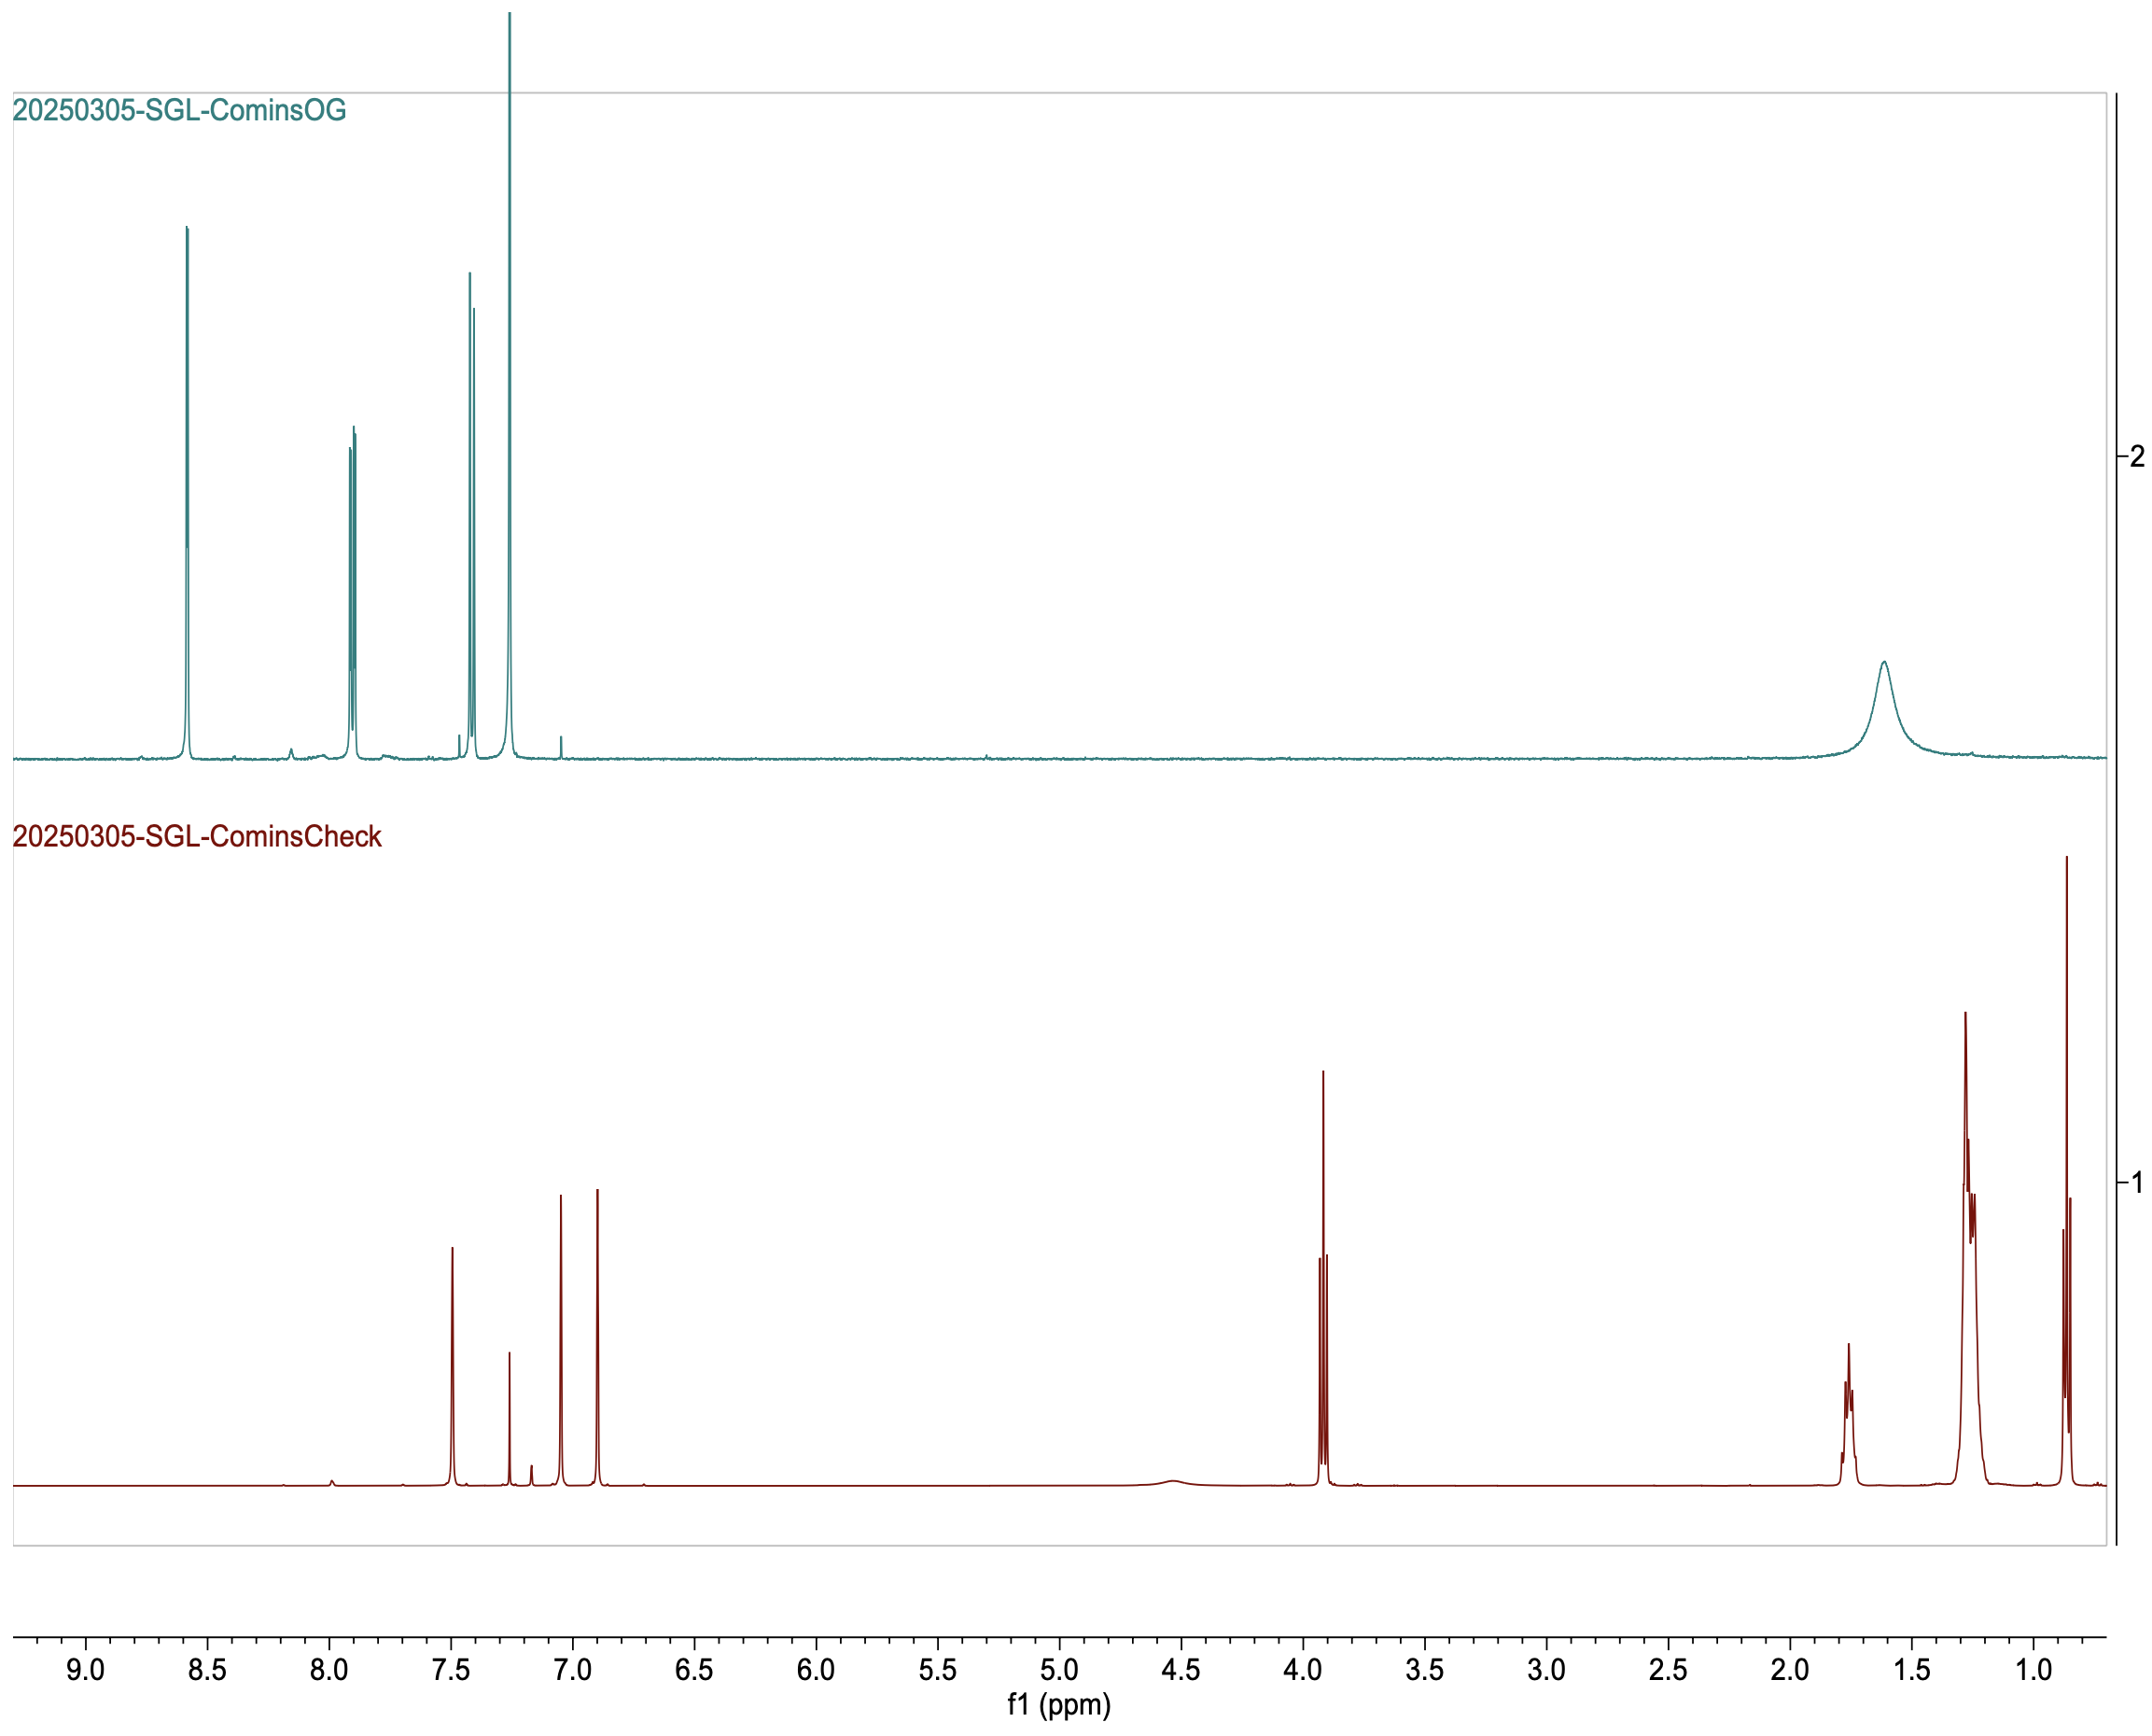
\includegraphics[width=\linewidth]{FPOrderedReceived.png}
    \caption{\ce{{}^1H} NMR of unknown (bottom) vs. what I ordered (top) in \ce{CDCl3}.}
    \label{fig:FPOrderedReceived}
\end{figure}
As such, for this project, I set out to characterize this compound using the techniques we've learned in 5.46.



\section{Pure or Mixture?}
The first thing I set out to do was determine if the substance I had received was pure. The initial \ce{{}^1H} NMR had several indistinct multiplets with unusual integrations, so I thought it was possible I had received a mixture of compounds. Thus, I ran a DOSY experiment (Figure \ref{fig:FPdosy}).
\begin{figure}[H]
    \centering
    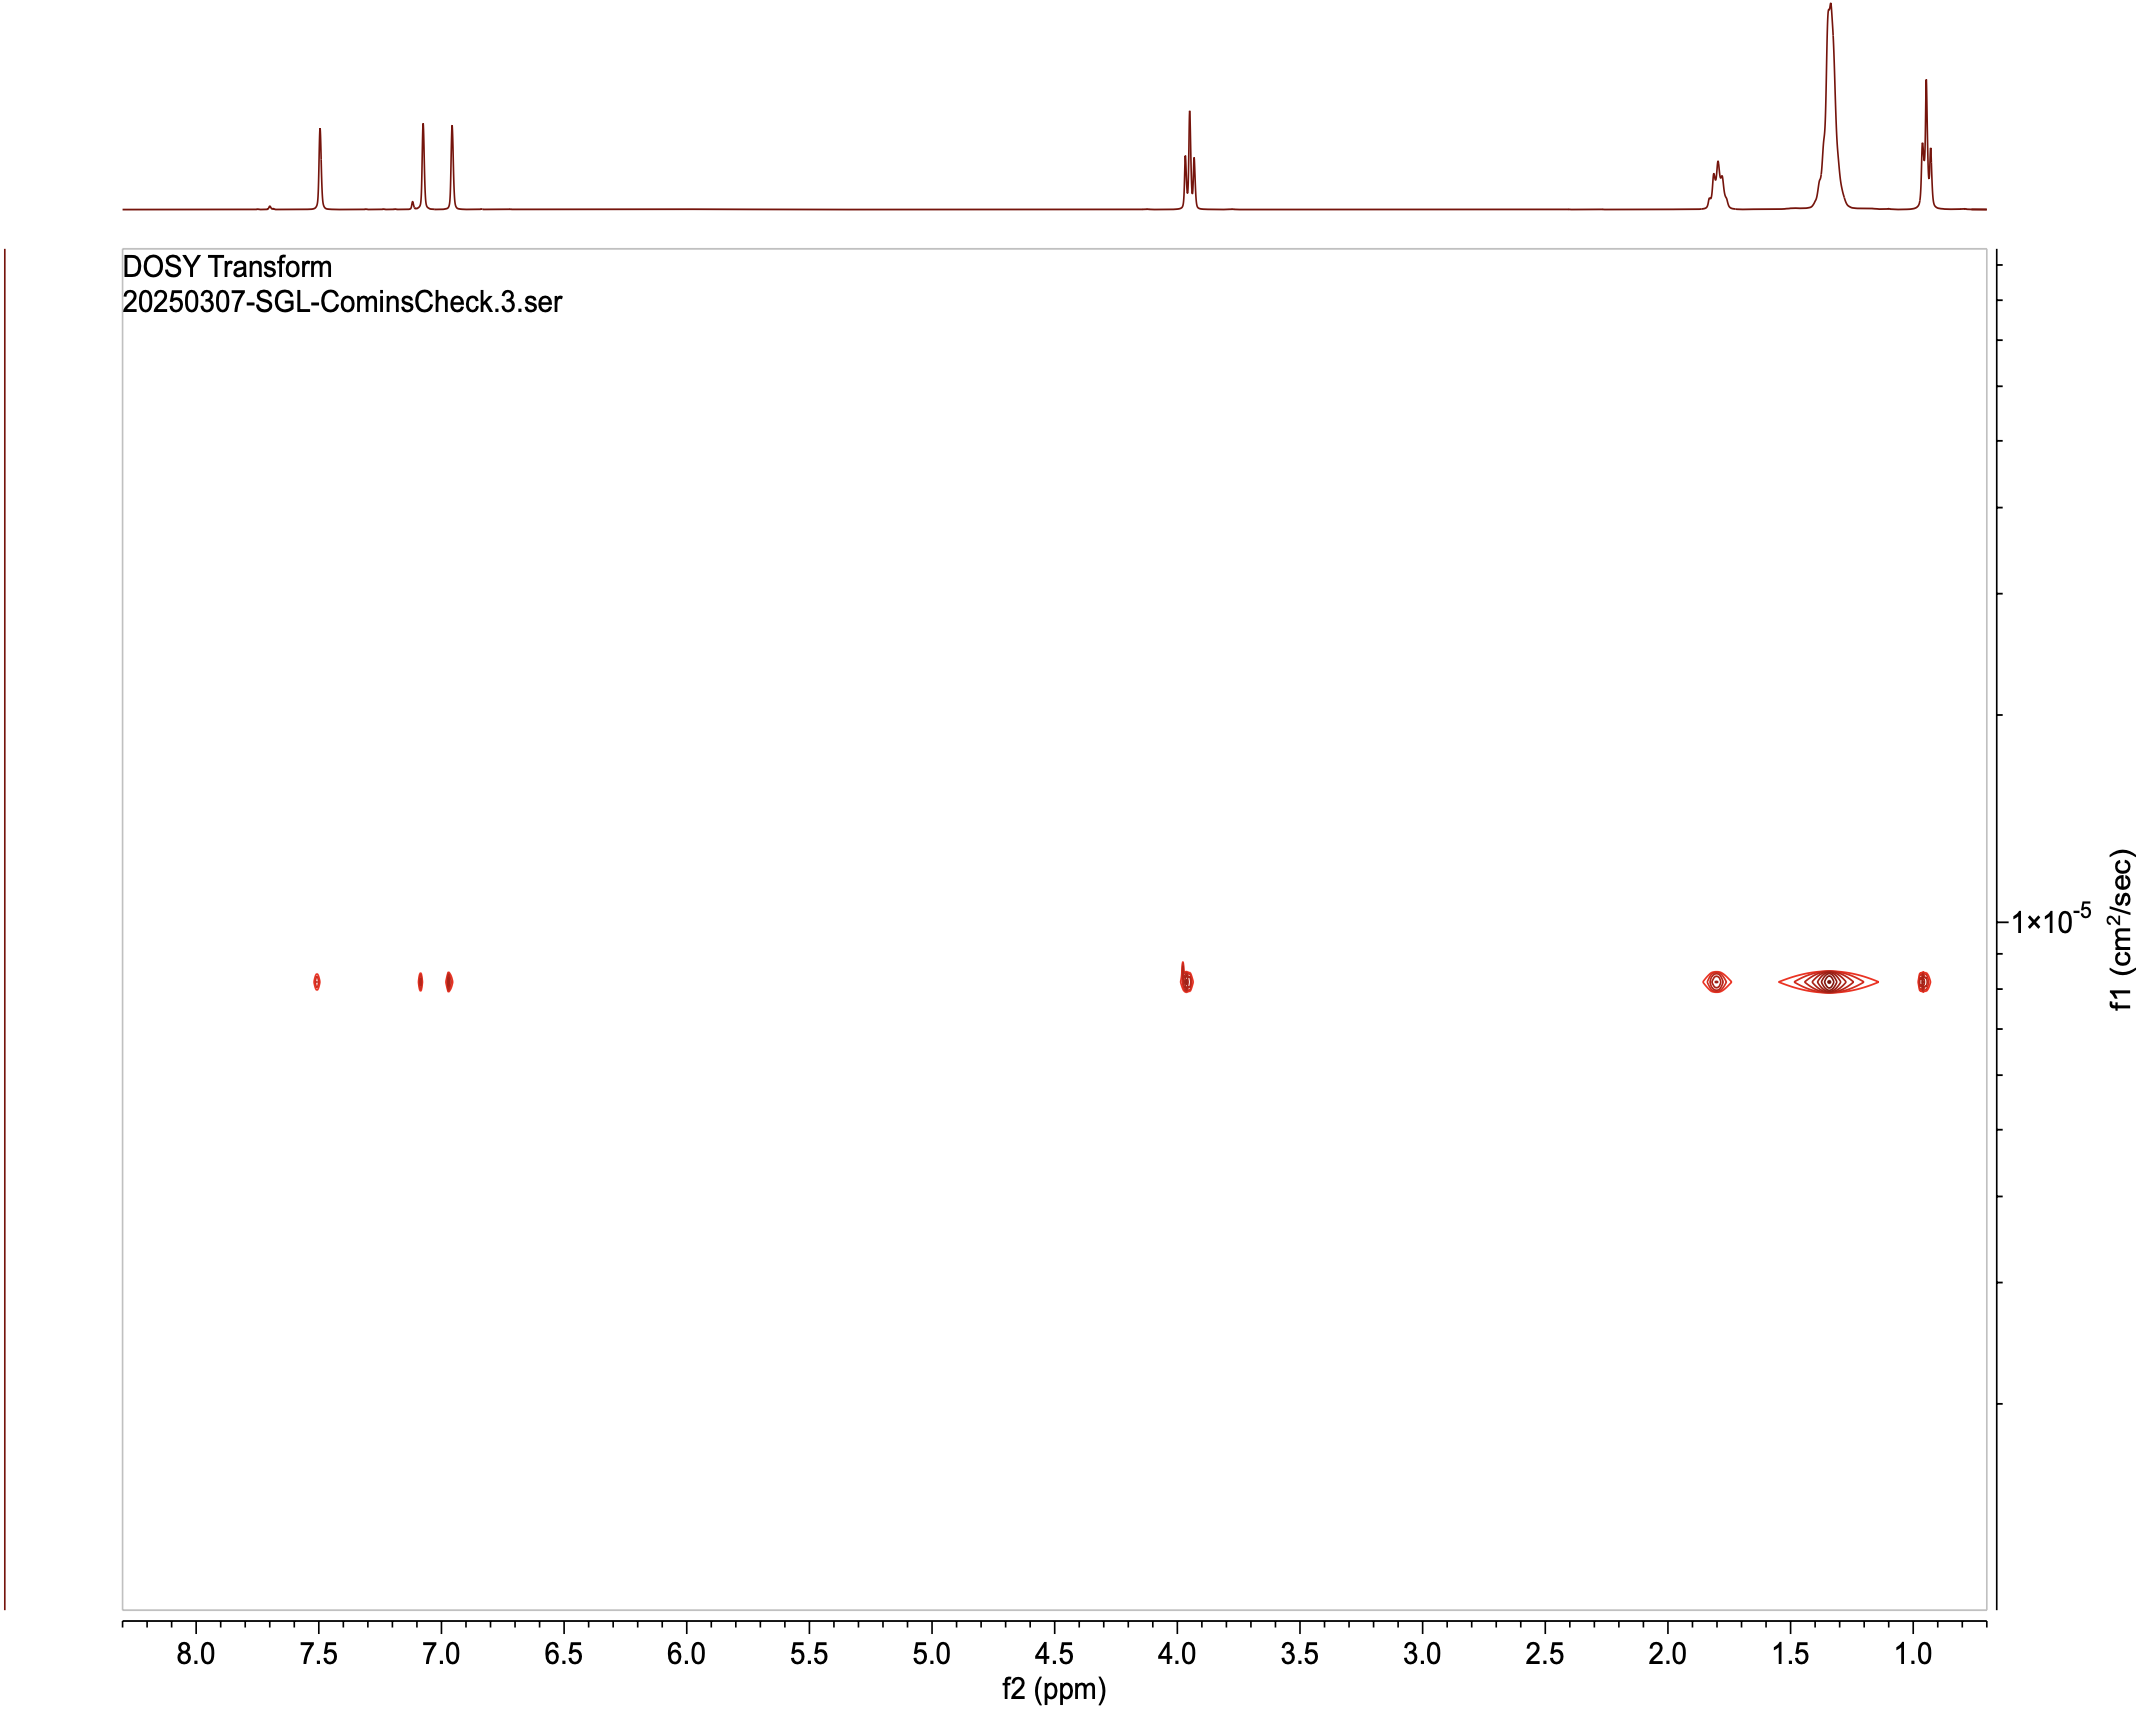
\includegraphics[width=\linewidth]{FPdosy.png}
    \caption{DOSY NMR spectrum of unknown.}
    \label{fig:FPdosy}
\end{figure}
Working up the DOSY data as a pseudo-2D spectrum in MNova, I observed a single horizontal line corresponding to the unknown compound. As to the few minor impurities visible in the \ce{{}^1H} NMR spectrum at the top of the DOSY, zooming in revealed that these impurities had distinct diffusion coefficients. As such, I neglected them from the remainder of my analysis. Note that I have not included a picture of the zoomed in spectrum, but it is available upon request.



\section{What Is It?}\label{sse:WhatIsIt}
To guide the remainder of my analysis, I began by running a standard method gas chromatography-mass spectrometry (GC-MS) experiment on a \SI[per-mode=symbol]{0.01}{\milli\gram\per\milli\liter} sample of the unknown compound. Consistent with my DOSY, only one big peak showed up in the GC-MS. It corresponded to the following mass spectrum.
\begin{figure}[H]
    \centering
    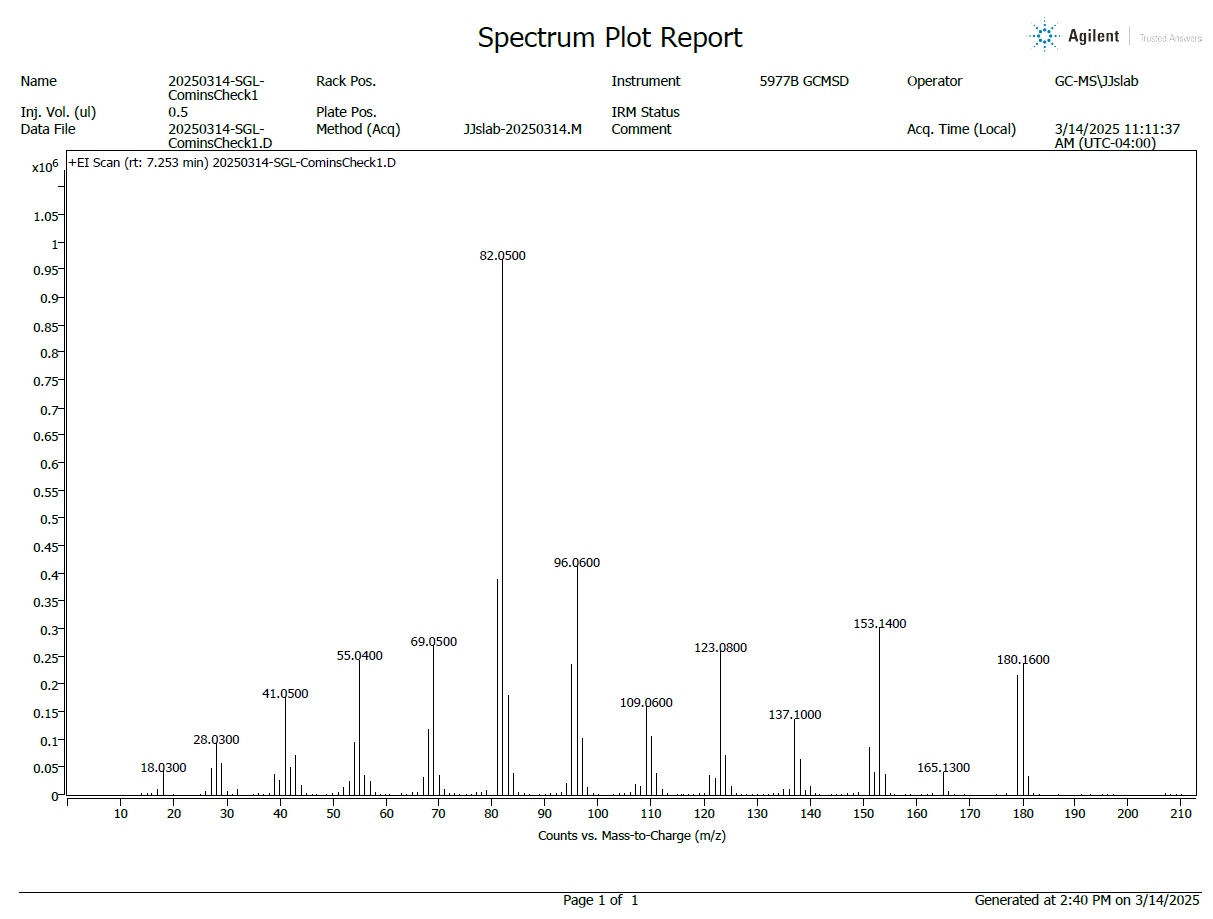
\includegraphics[width=\linewidth]{FPgcms.png}
    \caption{Mass spectrum of unknown.}
    \label{fig:FPgcms}
\end{figure}
Assuming that the peak at $m/z=179$ corresponded to loss of a proton and $m/z=181$ corresponded to the mono-\ce{{}^13C} isotopic variants of the unknown, I concluded that the parent peak (and thus, the molecular weight of the unknown) was $[\text{M}]=180$. The relative integrations of the $[\text{M}]$ and $[\text{M}+1]$ peaks, combined with the known isotopic abundance of \ce{{}^13C} at $1.1\%$ also suggested that there were
\begin{equation*}
    \frac{0.033}{0.241+0.033}\times\frac{100}{1.1} \approx 11
\end{equation*}
carbon atoms in the molecule. The general distribution of the fragment peaks --- several gaps of $m/z=14$ --- also suggested that a long chain of methylene (\ce{CH2}) groups was part of the molecule somehow. Lastly, the absence of $[\text{M}+2]$ peaks in a characteristic $3:1$ or $1:1$ ratio suggested that the unknown contained neither a chlorine nor a bromine heteroatom.\par
With these ideas in mind, I returned to the \ce{{}^1H} NMR spectrum to begin brainstorming ideas. From my summer research, I was somewhat familiar with the \ce{{}^1H} NMR spectra of long, saturated aliphatic chains. As such, with the hints from the mass spectrum, I now recognized the aliphatic peaks in Figure \ref{fig:FPOrderedReceived} as characteristic of an \emph{n}-octyl group attached to an electron-withdrawing group (EWG). Here's how. First, the four aliphatic peaks integrated in a $2:2:10:3$ ratio. The peak at \SI{3.95}{\partspermillion} was likely attached to the EWG (hence deshielded), and split into a triplet by the two adjacent protons. Specifically, these two adjacent protons would likely correspond to the apparent pentet at \SI{1.80}{\partspermillion}; they would be the next most deshielded, and their splitting would be due to their approximately equal coupling to the two \ce{CH2}'s on either side (bearing 4 protons, total). The broad multiplet at \SI{1.34}{\partspermillion} with integration 10 would then correspond to the five methylenes in the mushy middle of the \emph{n}-octyl chain, which are technically chemically distinct but close enough in chemical environment to overlap significantly. Lastly, the triplet at \SI{0.95}{\partspermillion} would likely correspond to the terminal methyl group on the \emph{n}-octyl chain, with integration 3, splitting caused by the sole adjacent \ce{CH2}, and significant roofing toward the multiplet. To help visualize this explanation, the reader should feel free to look ahead to the final peak assignments in Figure \ref{fig:FP1H}.\par
With the aliphatic region assigned, the only remaining question was the nature of the EWG. From the proton spectrum, there remained three apparent singlets in the aromatic region, integrating in a $1:1:1$ ratio. This suggested that the EWG was aromatic and at least partially asymmetric. From the mass spectrum, I had (subtracting out the \emph{n}-octyl group) $11-8=3$ carbons and $180-113=\SI[per-mode=symbol]{67}{\gram\per\mole}$ of mass for which to account. Subtracting out the three carbons and three aromatic protons left $67-39=\SI[per-mode=symbol]{28}{\gram\per\mole}$, or the mass of two nitrogen atoms. Thus, I concluded that the electron-withdrawing group was a 5-membered, $\pi$-deficient aromatic heterocycle of molecular formula \ce{C3H3N2}. Moreover, I concluded based on the significant downfield shift of the \emph{n}-octyl group's first methylene (\SI{3.95}{\partspermillion}) and the relatively thin linewidth of all aromatic protons (e.g., no exchange broadening) that this heterocycle was bonded to the \emph{n}-octyl group through one of its nitrogens.\par
This analysis narrowed the possible EWGs down to two: An \emph{N}-imidazolyl or \emph{N}-pyrazolyl group.
\begin{figure}[H]
    \centering
    \footnotesize
    \begin{subfigure}[b]{0.45\linewidth}
        \centering
        \chemfig{-[:30]-[:-30]-[:30]-[:-30]-[:30]-[:-30]-[:30]-[:-30]N*5(-=-N=-)}
        \caption{1-octylimidazole.}
        \label{fig:FPOcIma}
    \end{subfigure}
    \begin{subfigure}[b]{0.45\linewidth}
        \centering
        \chemfig{-[:30]-[:-30]-[:30]-[:-30]-[:30]-[:-30]-[:30]-[:-30]N*5(-=-=N-)}
        \caption{1-octylpyrazole.}
        \label{fig:FPOcImb}
    \end{subfigure}
    \caption{The final candidates.}
    \label{fig:FPOcIm}
\end{figure}
Now, I searched the literature for reported \ce{{}^1H} NMR spectra of 1-octylimidazole\supercite{bib:FPOcIm} and 1-octylpyrazole.\supercite{bib:FPOcPz} The unknown's chemical shifts matched those of 1-octylimidazole perfectly up to referencing. Of note was the match with the imidazole moiety's characteristically downshifted C2 proton (between the imidazole's two nitrogens). However, I could only find one reported \ce{{}^1H} NMR spectrum for 1-octylpyrazole (in \ce{CCl4}, from the '80s). Even considering these limitations, it did not seem to be nearly as good a fit. As such, I proposed that the unknown is \fbox{1-octylimidazole.}
\newpage



\section{Confirming the Proposed Structure}\label{sse:Confirm}
If the unknown is 1-octylimidazole, its \ce{{}^13C} NMR spectrum should have 11 distinct carbon peaks, as the mass spectrum suggested. Using a \SI{300}{\milli\gram} sample in \SI{0.7}{\milli\liter} of \ce{CDCl3} and a high-field instrument to obtain a good signal-to-noise ratio without resorting to excessive number of scans, I collected a \ce{{}^13C} NMR spectrum of the unknown (Figure \ref{fig:FP13C}).
\begin{figure}[H]
    \centering
    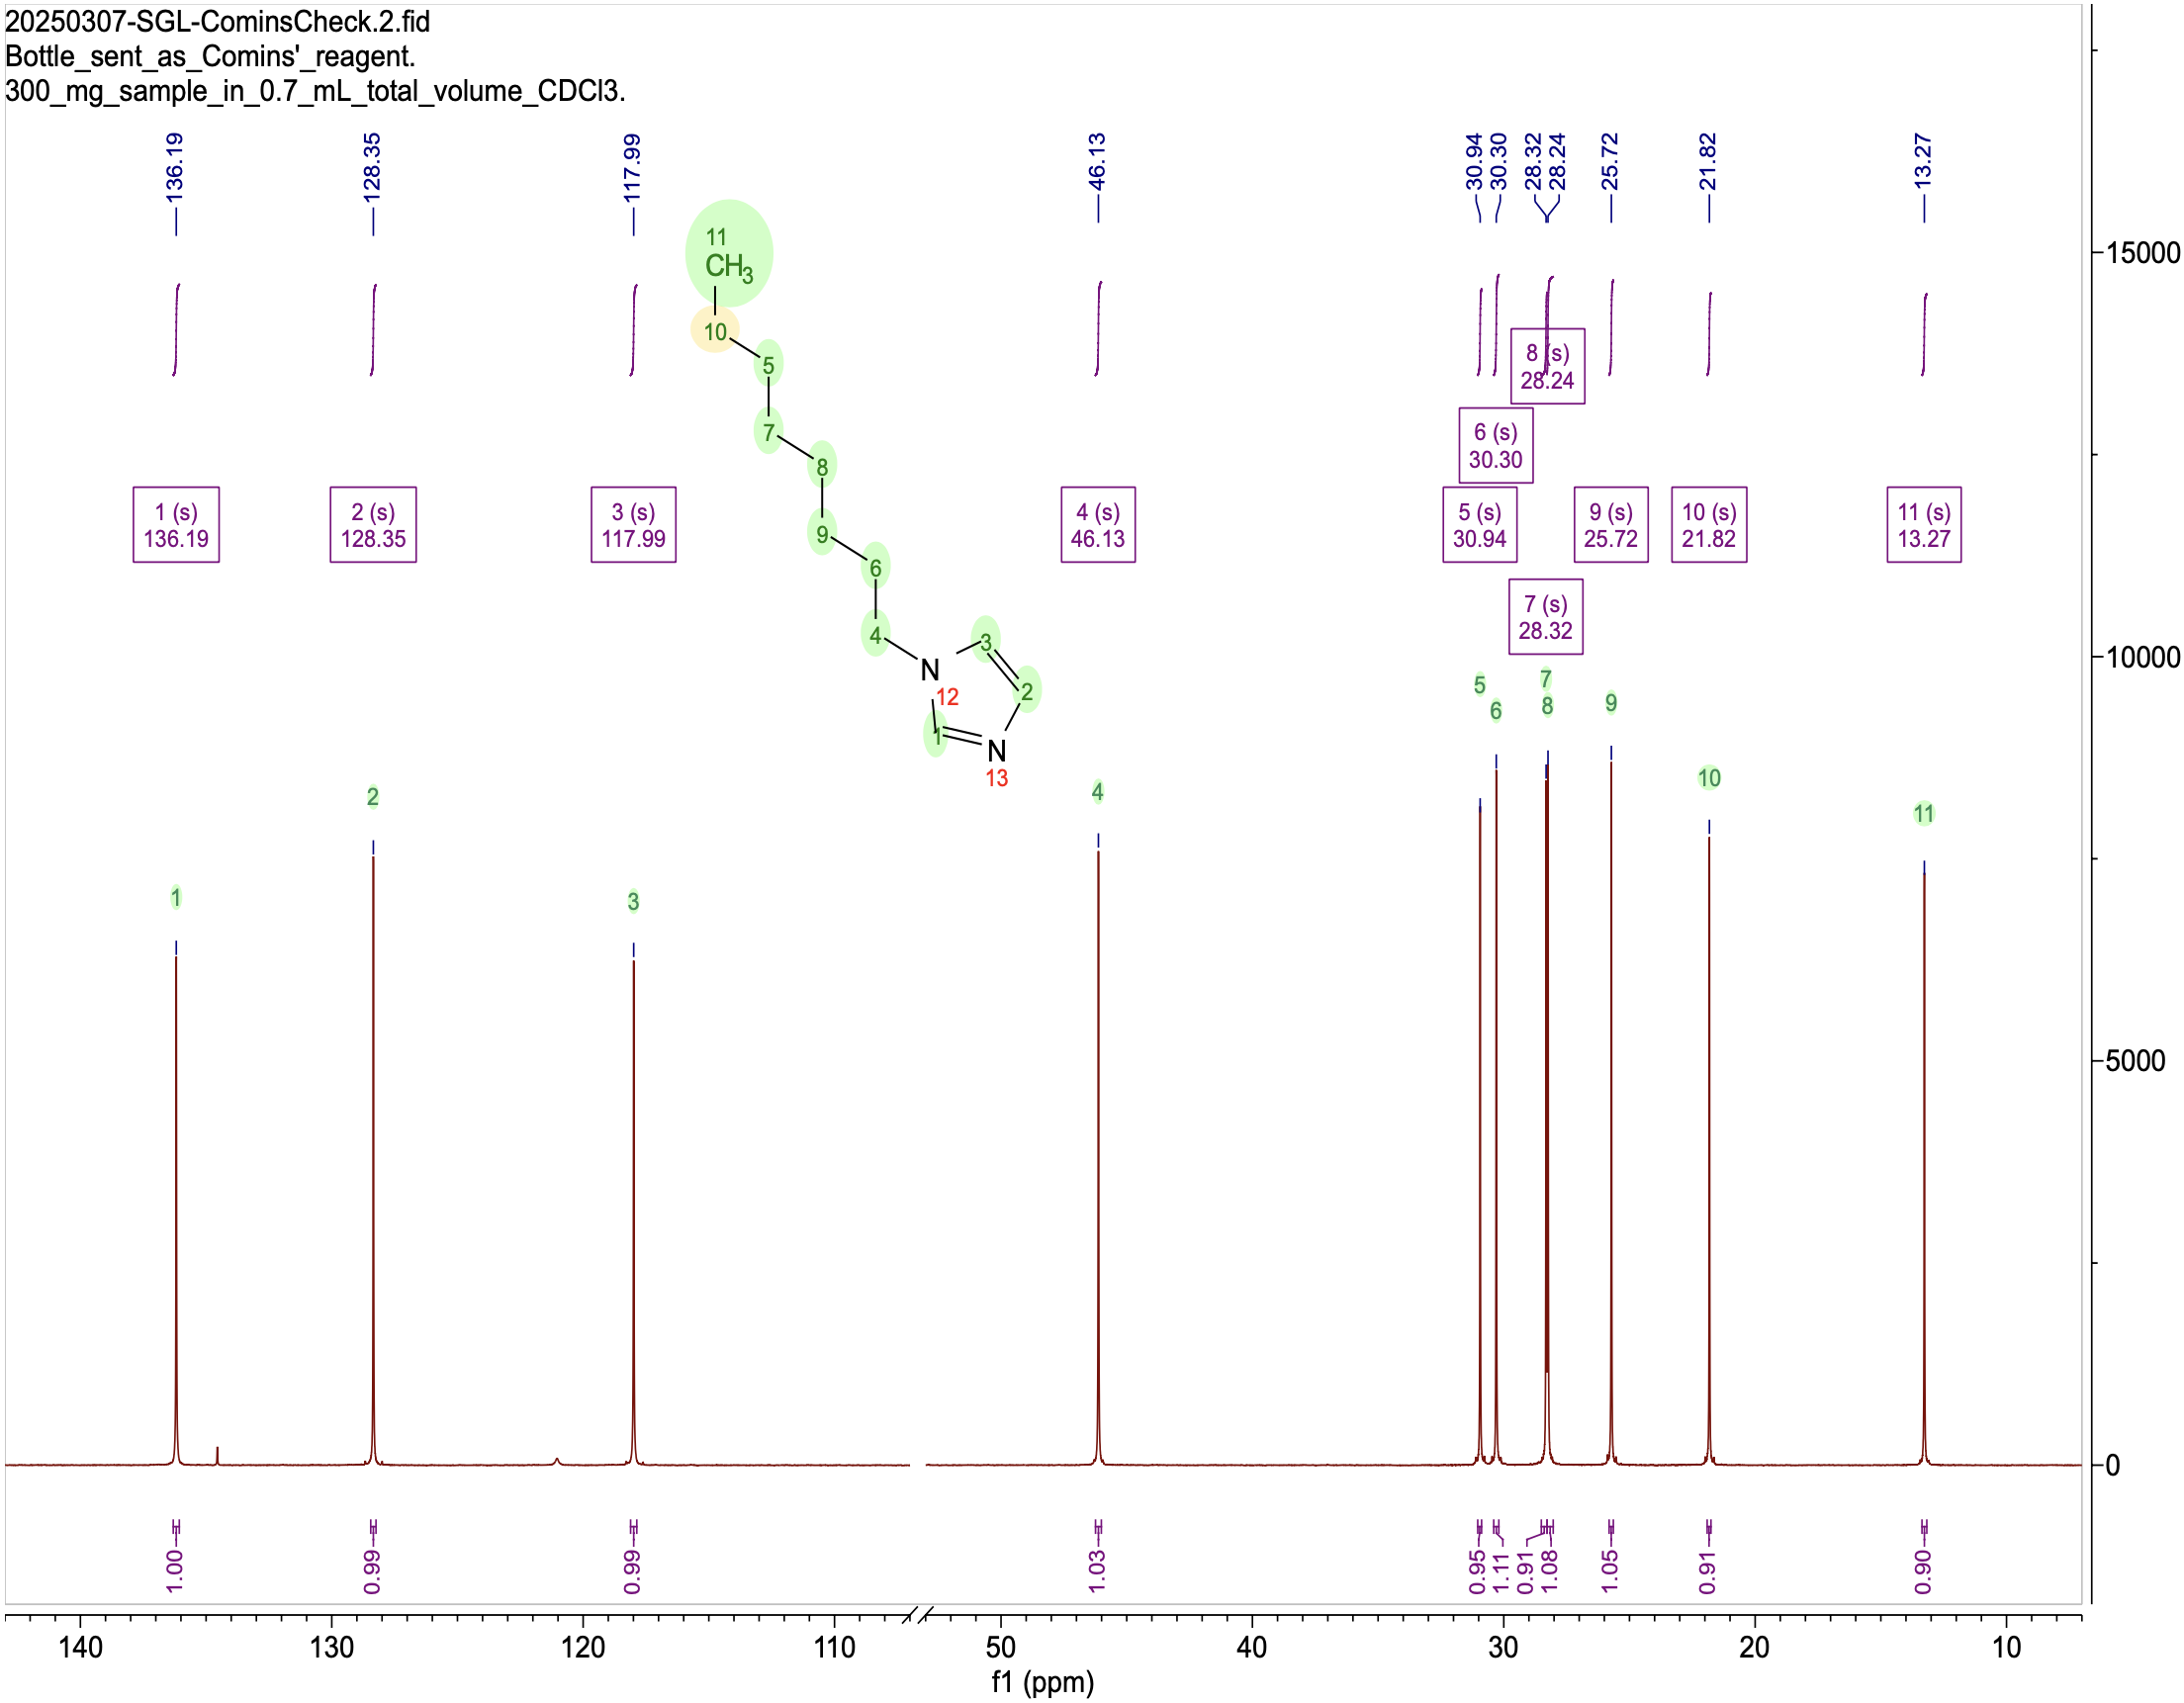
\includegraphics[width=\linewidth]{FP13C.png}
    \caption{\ce{{}^13C} NMR spectrum of unknown.}
    \label{fig:FP13C}
\end{figure}
It did indeed have 11 distinct peaks. Moreover, three of these peaks fell in the aromatic region, and eight of them fell in the aliphatic region (also as expected). Note that the peak assignments in Figure \ref{fig:FP13C} are \emph{not} self-explanatory, and the experimental evidence I collected to assign them will be discused much more below. That being said, their order does line up perfectly with MNova's predicted \ce{{}^13C} spectrum for 1-octylimidazole. Thus, it is possible that for a quick and dirty approach to peak assignments, we may not need any more experimental evidence than this.
\newpage


Let's move on. If the unknown is 1-octylimidazole, its COSY spectrum should enable the viewer to "walk" down the aliphatic region and to see each aromatic peak coupled each other aromatic peak (through either vicinal or W-coupling). To test these hypotheses, I collected the following \ce{{}^1H}-\ce{{}^1H} COSY spectrum.
\begin{figure}[H]
    \centering
    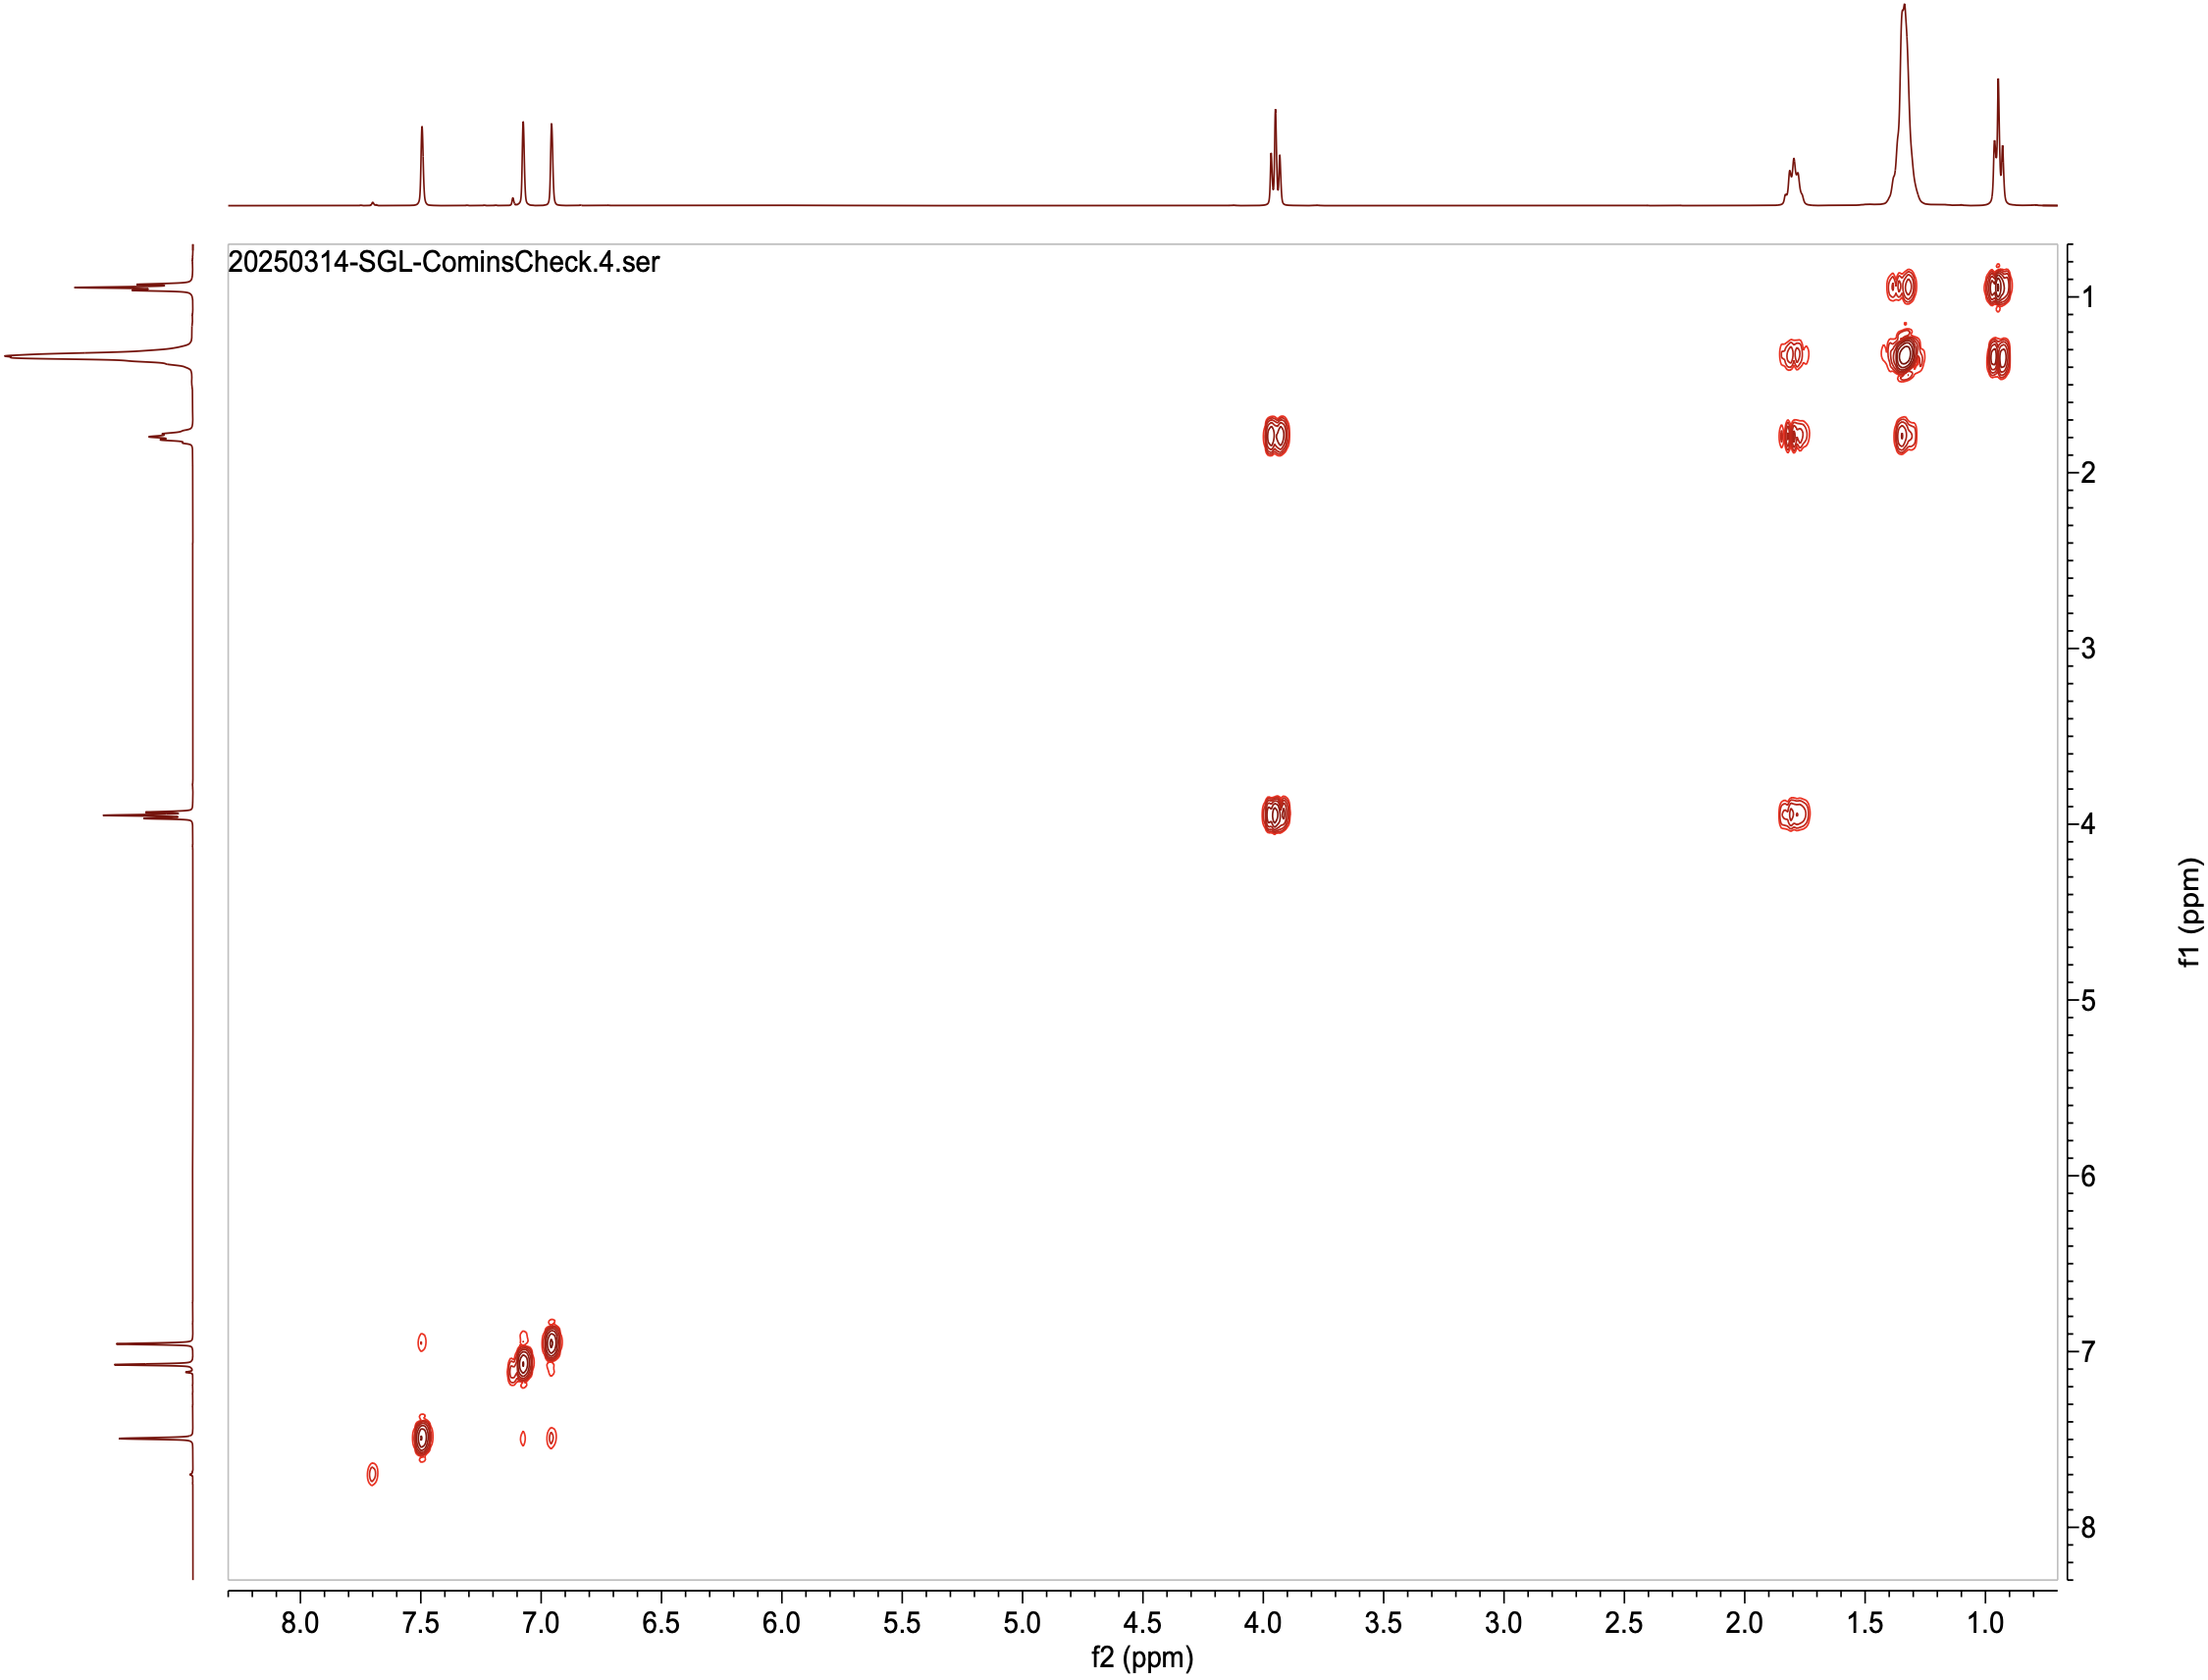
\includegraphics[width=\linewidth]{FPcosy.png}
    \caption{\ce{{}^1H}-\ce{{}^1H} COSY NMR spectrum of unknown.}
    \label{fig:FPcosy}
\end{figure}
First off, note that the diagonal cross peak at \SI{7.70}{\partspermillion} corresponds to one of the impurities identified by the aforementioned zoomed-in DOSY; thus, it should be neglected. With that out of the way, observe that --- as expected --- all aromatic peaks resonate with one another (see the bottom-left corner of the spectrum). Specifically, each peak has cross peaks with every other peak. Additionally, in the upper-right hand region, we can "walk" from the diagonal peak at \SI{3.95}{\partspermillion}, up to the cross peak at $(\SI{3.95}{\partspermillion},\SI{1.80}{\partspermillion})$, right to the diagonal peak at \SI{1.80}{\partspermillion}, up to the cross peak at $(\SI{1.80}{\partspermillion},\SI{1.34}{\partspermillion})$, right to the diagonal peak at \SI{1.34}{\partspermillion}, up to the cross peak at $(\SI{1.34}{\partspermillion},\SI{0.95}{\partspermillion})$, and right to the diagonal peak at \SI{0.95}{\partspermillion}. Note that the splitting of some of the COSY peaks is likely a reflection of the splitting in the \ce{{}^1H} NMR peaks, not a distinct phenomenon.
\newpage


Moving on again, if the unknown is 1-octylimidazole, a DEPT 135-type experiment should have positively phased peaks in the aromatic region (\ce{CH}) and for the terminal methyl group (\ce{CH3}), and negatively phased peaks everywhere else (\ce{CH2}). Although I did not directly collect a DEPT 135 spectrum, I did indirectly collect one through a \ce{{}^1H}-\ce{{}^13C} HSQC (Figure \ref{fig:FPhsqc}).
\begin{figure}[H]
    \centering
    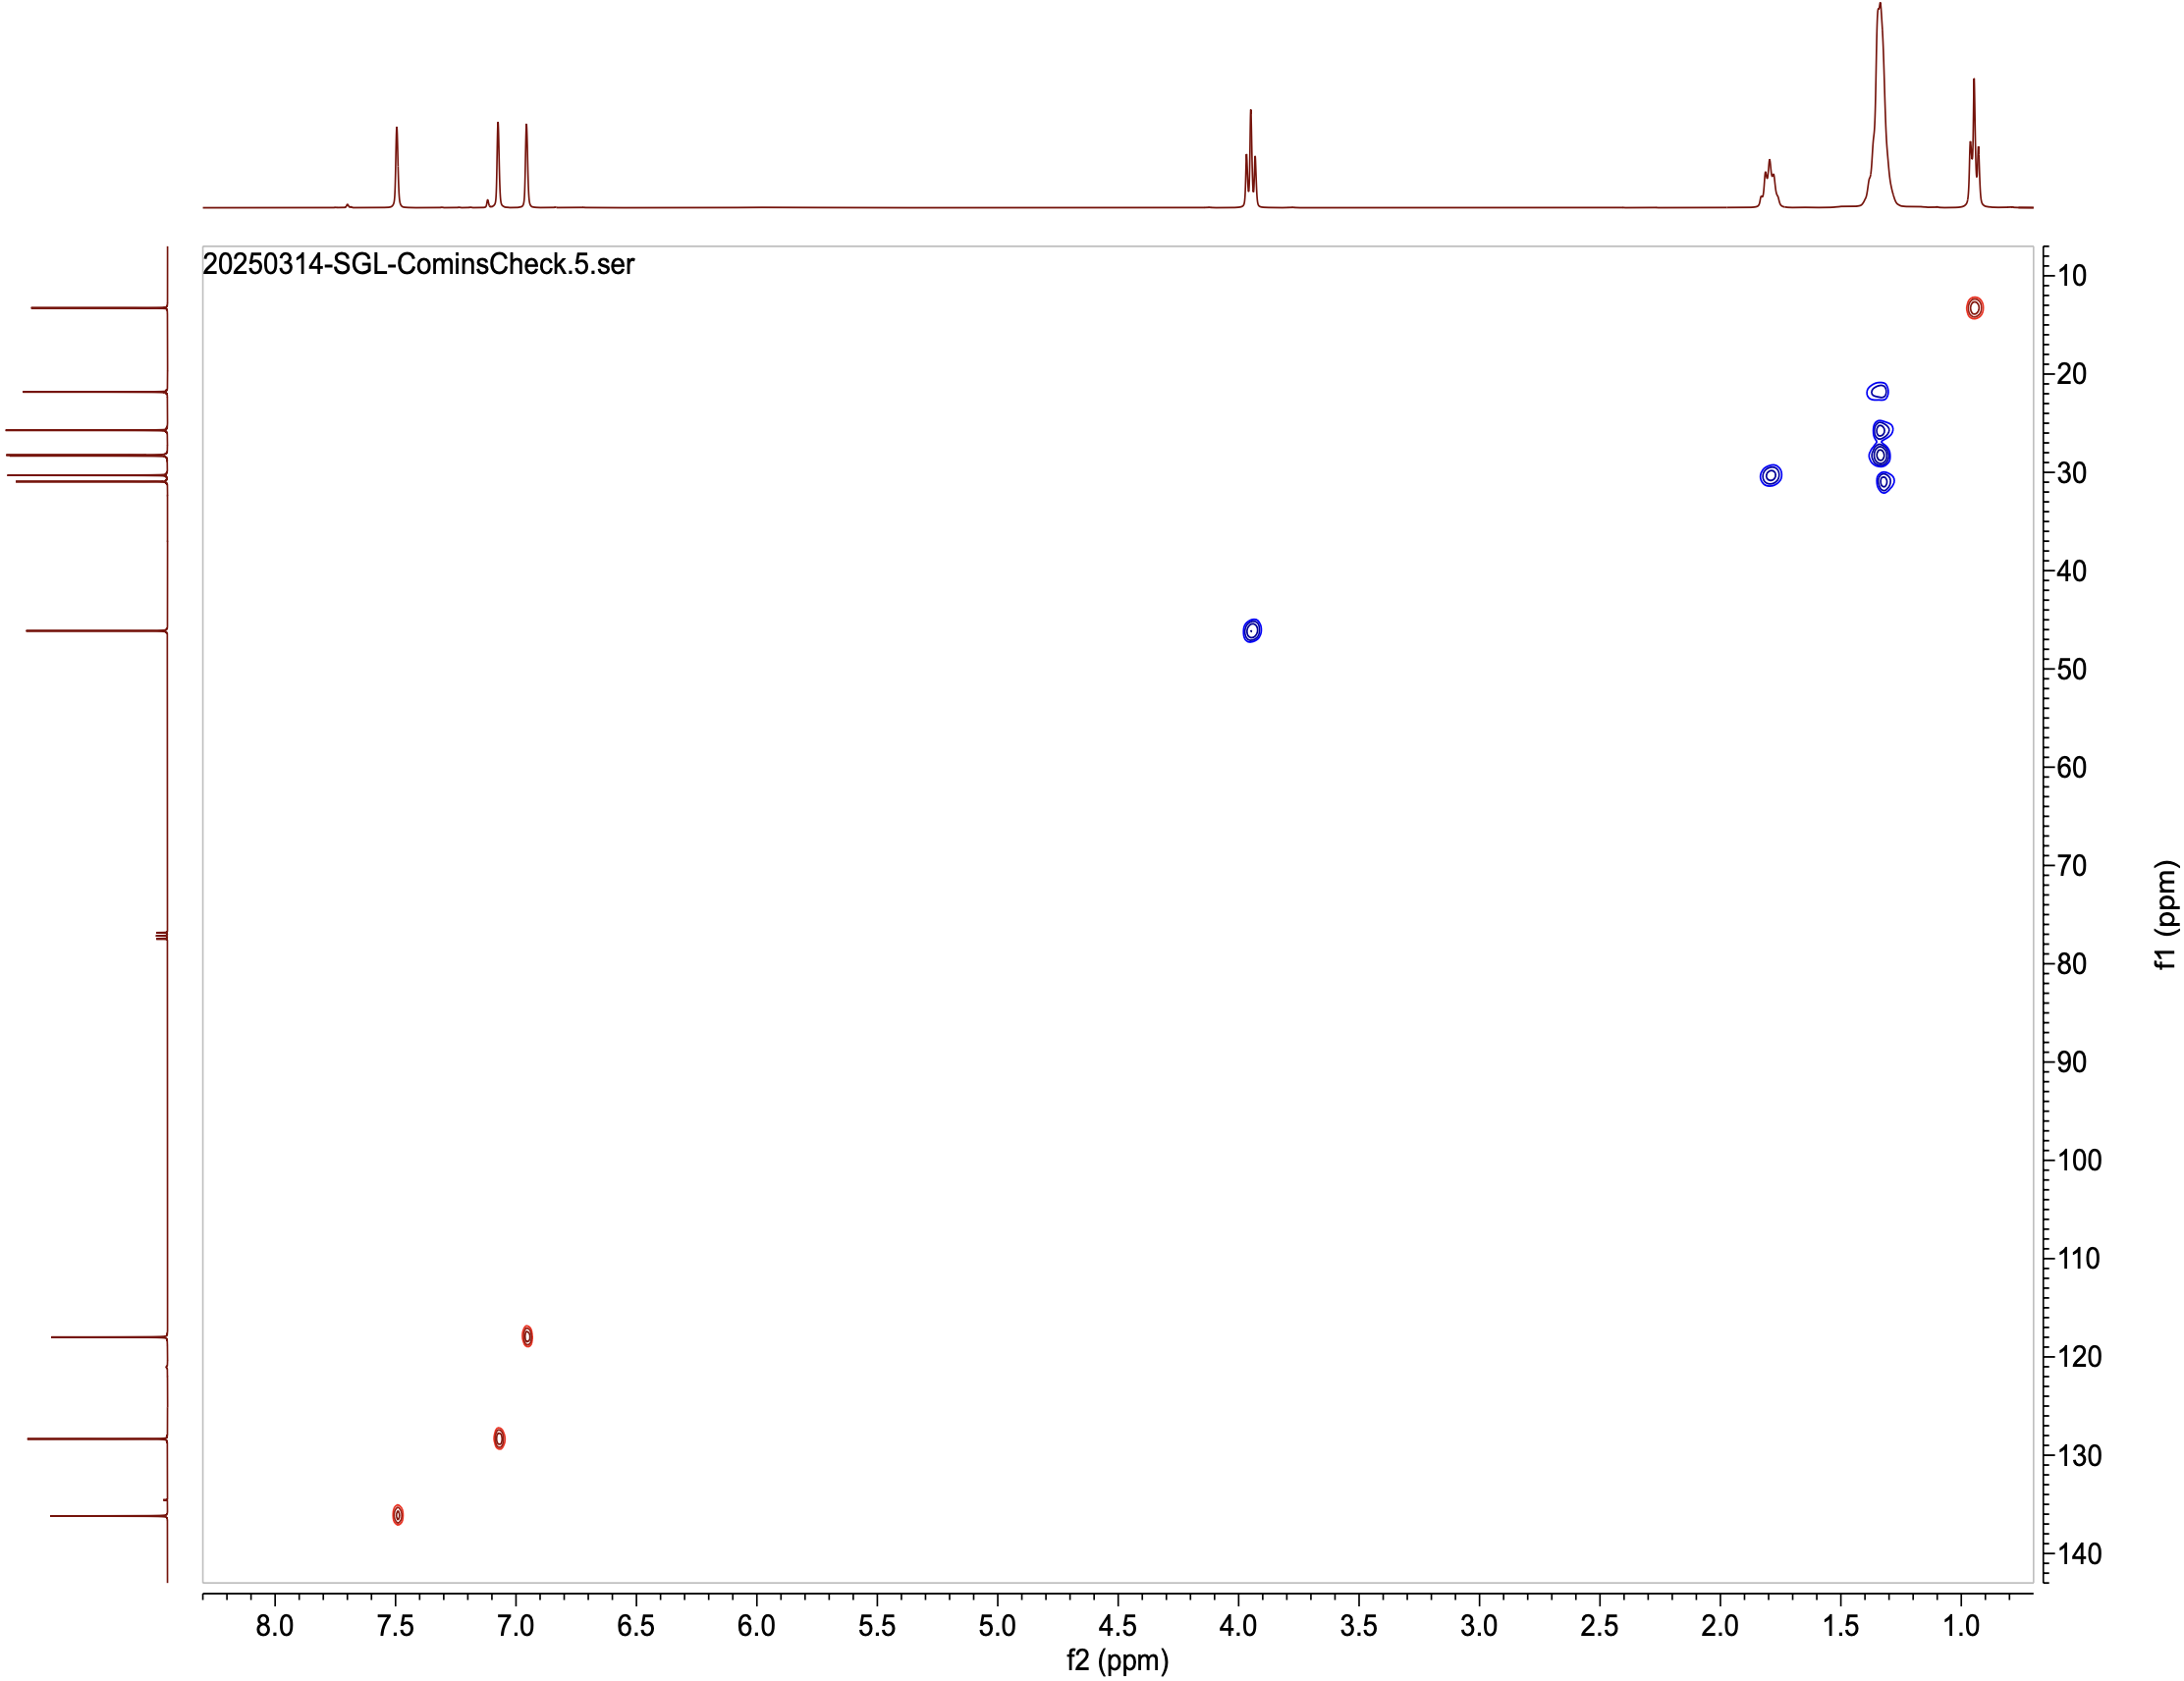
\includegraphics[width=\linewidth]{FPhsqc.png}
    \caption{\ce{{}^1H}-\ce{{}^13C} HSQC NMR spectrum of unknown.}
    \label{fig:FPhsqc}
\end{figure}
We do, indeed, see the anticipated phasing. Note that two carbon peaks (7 and 8 in Figure \ref{fig:FP13C}) heavily overlap, so these peaks overlap as well in Figure \ref{fig:FPhsqc} above to create a single blue peak of greater than normal intensity at $(\SI{1.34}{\partspermillion},\SI{28.26}{\partspermillion})$.
\newpage


Lastly, if the unknown is 1-octylimidazole instead of 1-octylpyrazole, the \SI{3.95}{\partspermillion} proton row in its \ce{{}^1H}-\ce{{}^13C} HMBC spectrum should have \emph{two} three-bond cross peaks with aromatic carbons (specifically, those labeled 1 and 3 in Figure \ref{fig:FP13C}) instead of \emph{one}. I anticipated that this experiment would serve as a "smoking gun" to resolve the imidazole/pyrazole debate, as opposed to the looser chemical shift argument given above.
\begin{figure}[H]
    \centering
    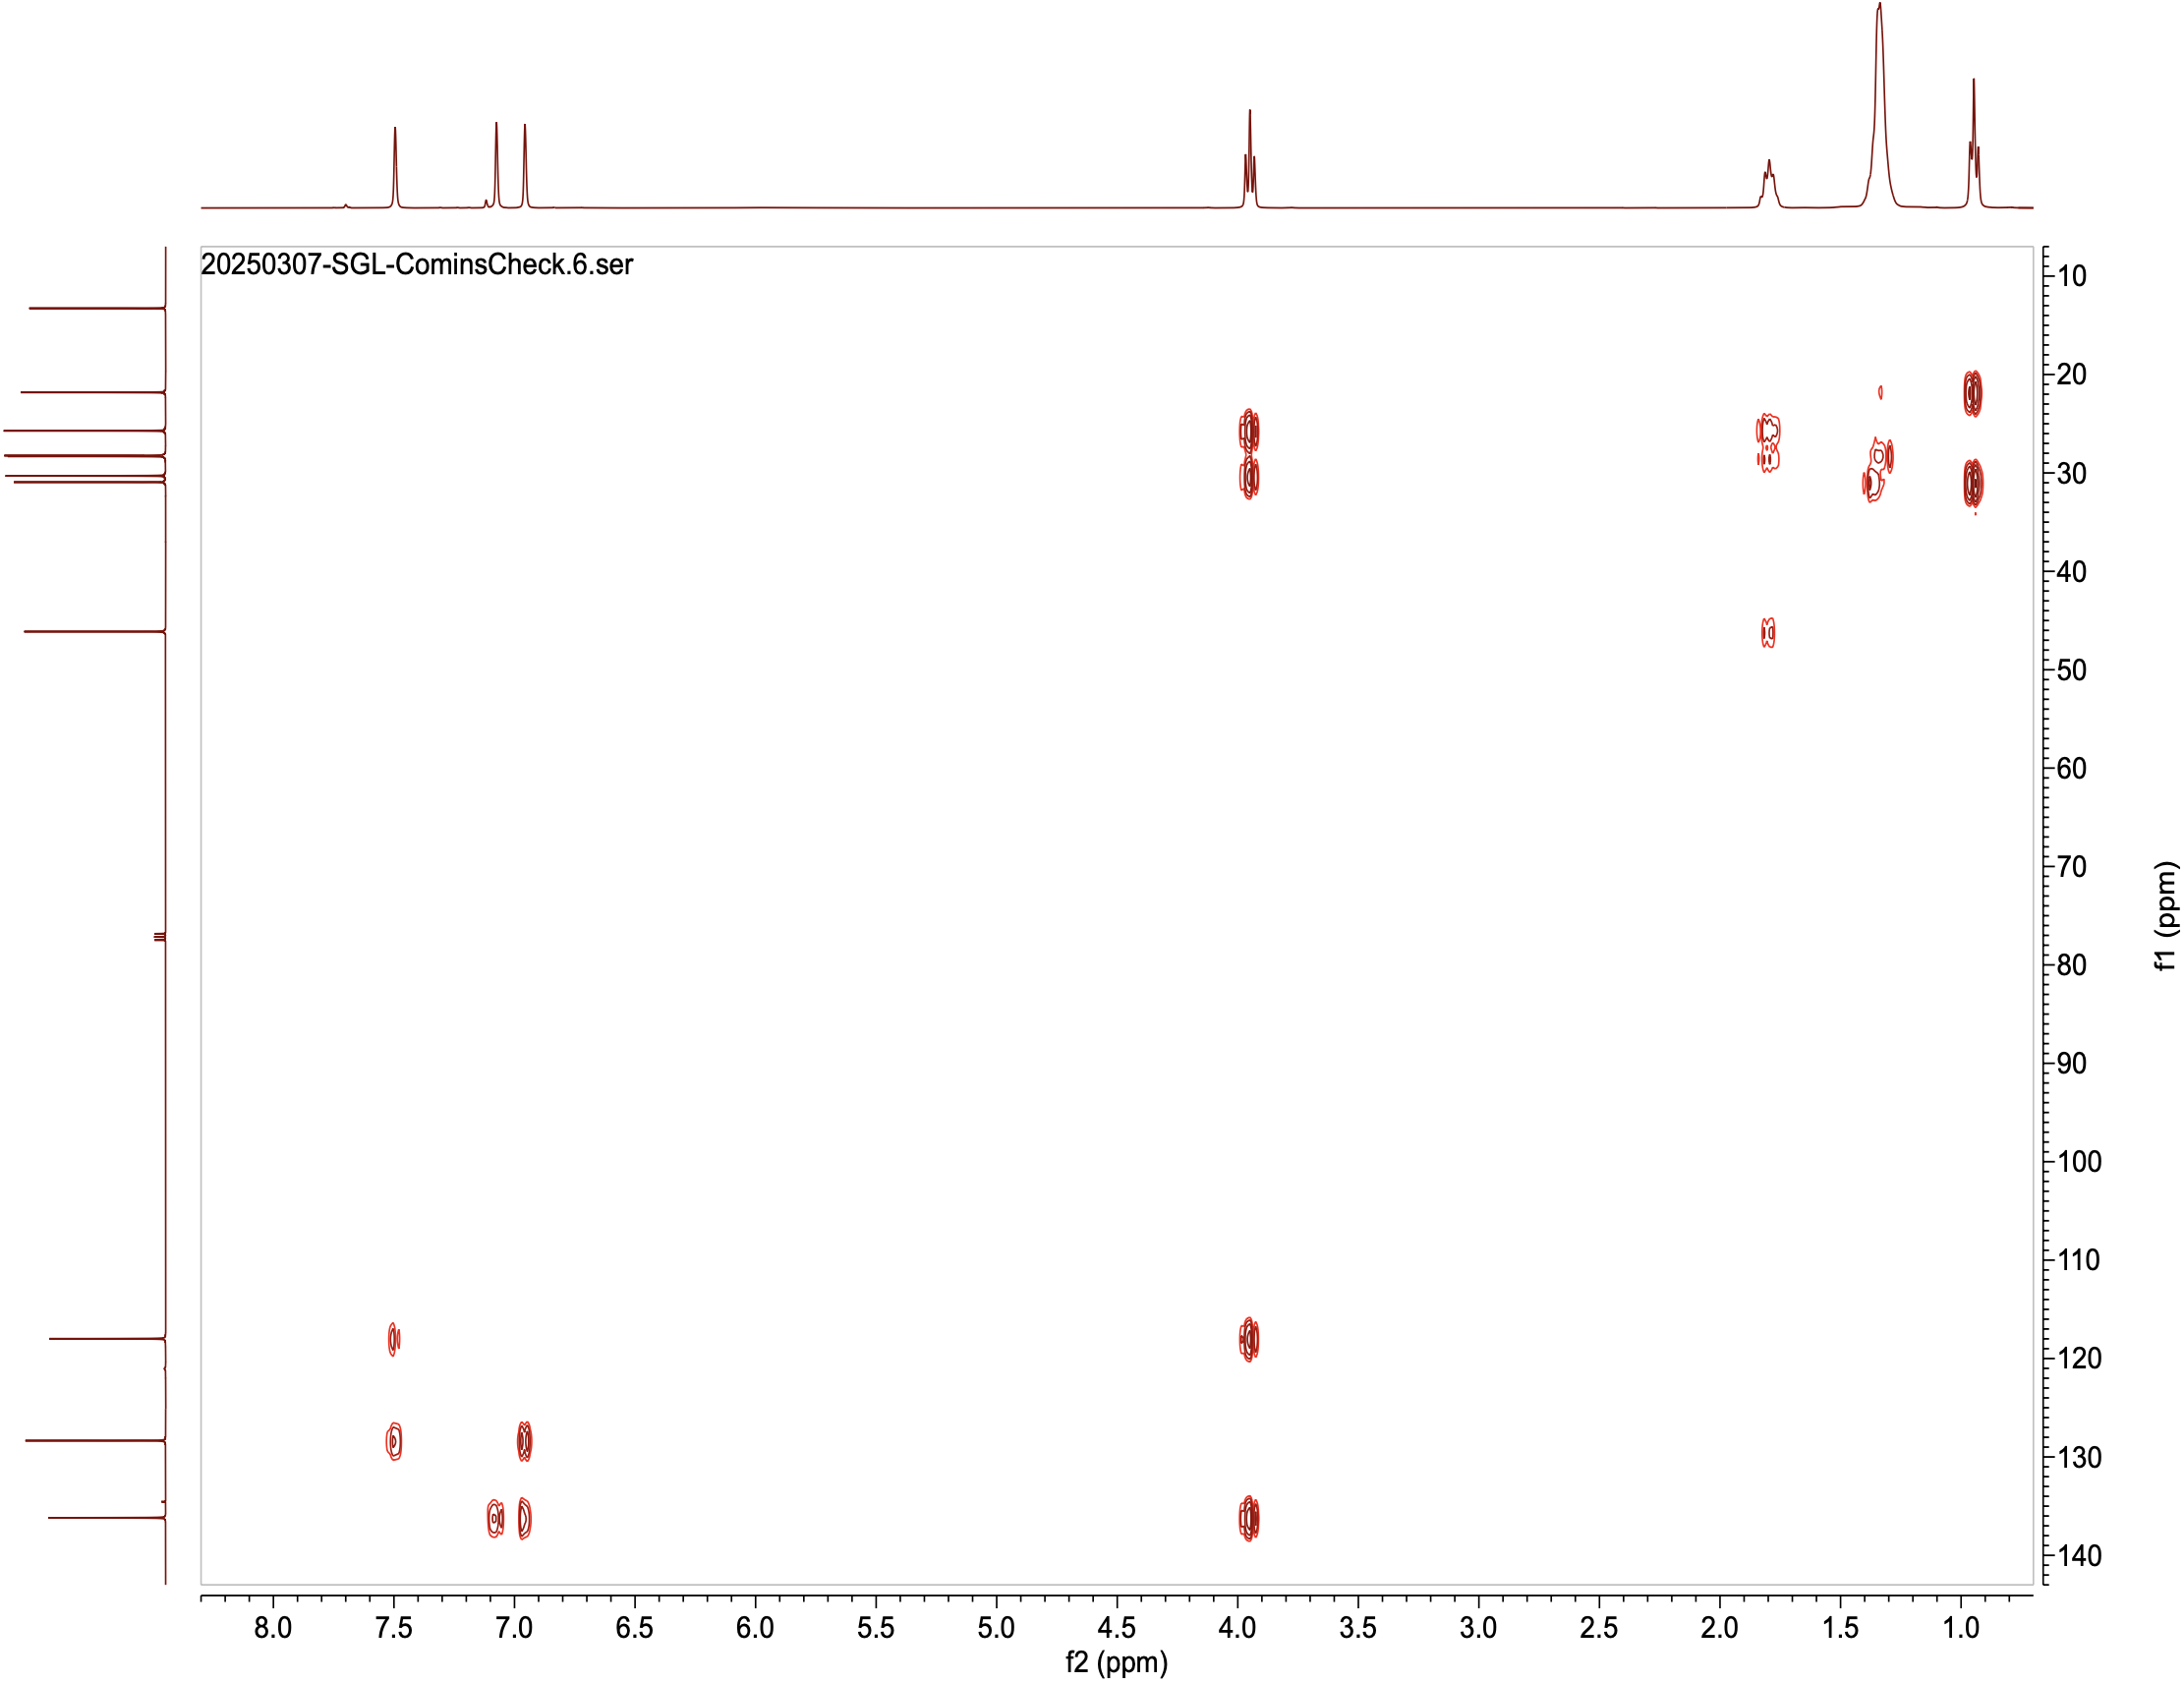
\includegraphics[width=\linewidth]{FPhmbc.png}
    \caption{\ce{{}^1H}-\ce{{}^13C} HMBC NMR spectrum of unknown.}
    \label{fig:FPhmbc}
\end{figure}
Indeed, there are two crosspeaks at $(\SI{3.95}{\partspermillion},\SI{117.99}{\partspermillion})$ and $(\SI{3.95}{\partspermillion},\SI{136.19}{\partspermillion})$. Thus, the compound almost certainly contains an imidazolyl moiety.\par
Note that the spectra shown above in this section could be interpreted to a much greater extent for structure confirmation purposes, but I'll leave such discussions to the next section on assigning the peaks.
\newpage



\section{Assigning Peaks}
I began by assigning some of the proton peaks with distinct chemical shifts.
\begin{figure}[H]
    \centering
    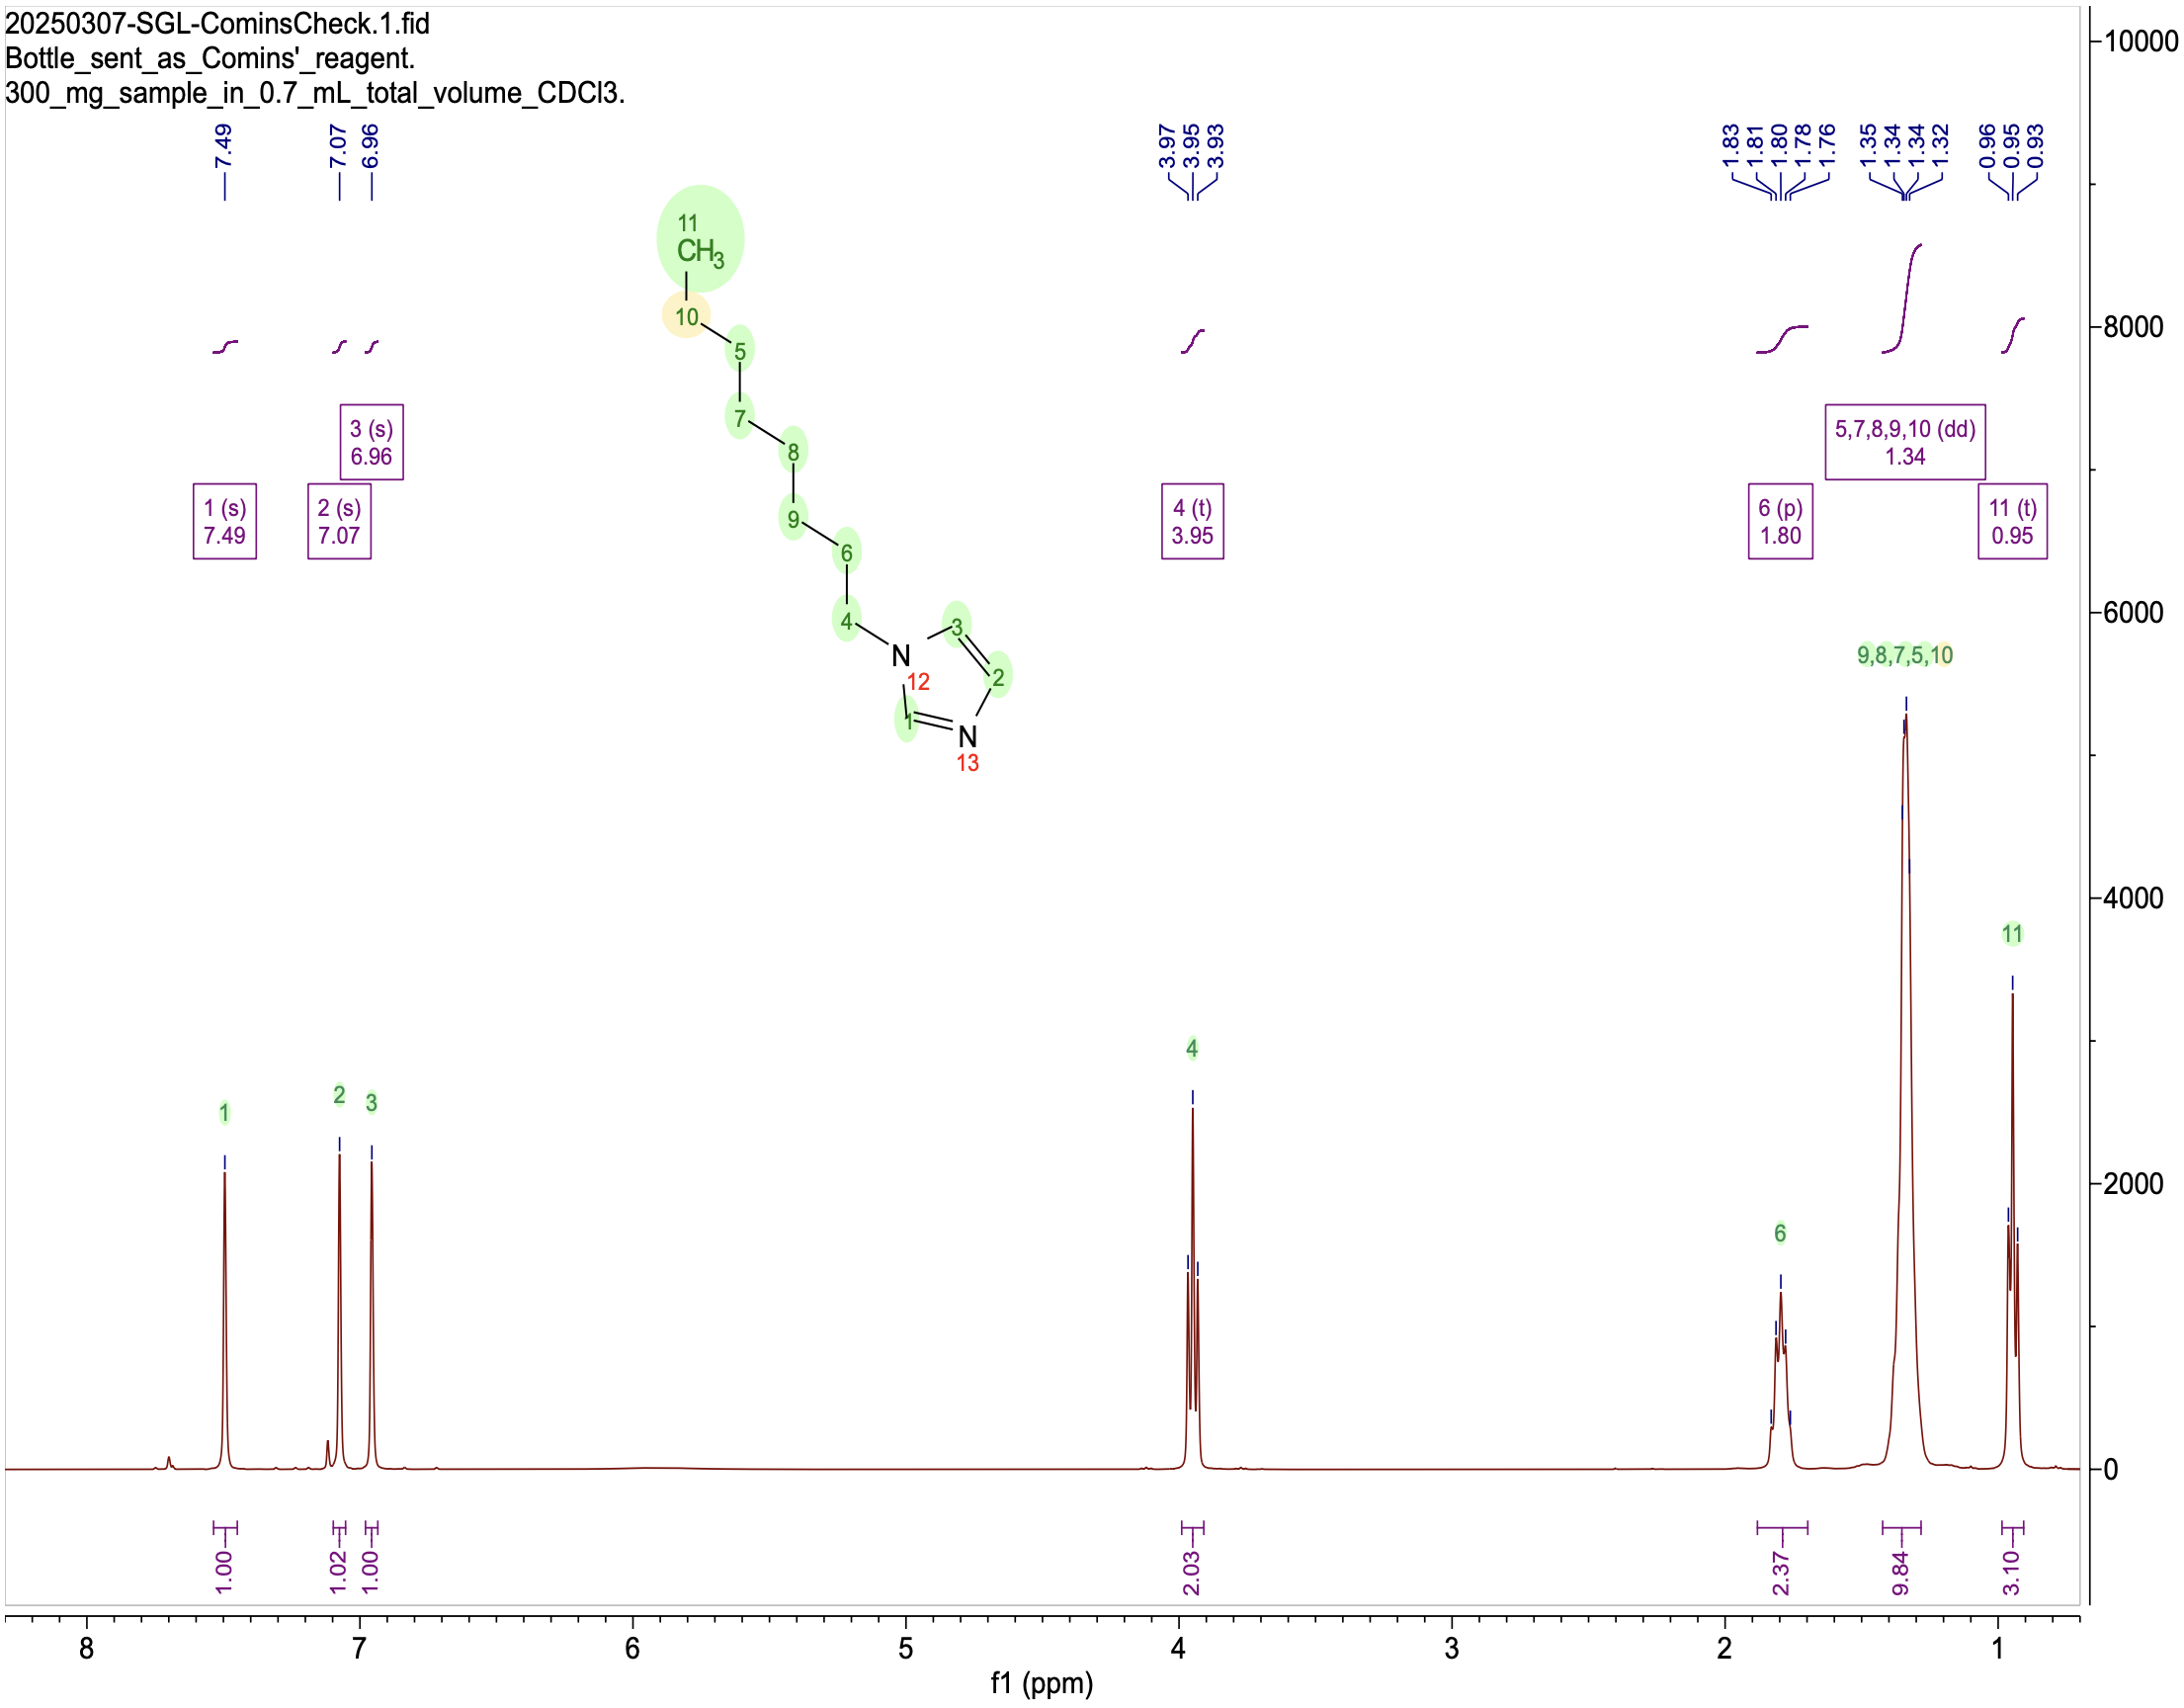
\includegraphics[width=\linewidth]{FP1H.png}
    \caption{\ce{{}^1H} NMR spectrum of unknown.}
    \label{fig:FP1H}
\end{figure}
Specifically, I assigned the \ce{{}^1H} peaks now named 4, 6, and 11 in the aliphatic region based on arguments made in Section \ref{sse:WhatIsIt}. I then assigned their corresponding carbon peaks (see Figure \ref{fig:FP13C}) based on the HSQC correlations (see Figure \ref{fig:FPhsqc}).\par
Next, I assigned the \ce{{}^13C} peaks now named 1 and 3 based on two pieces of evidence. First, I used the HMBC correlations to the proton now named 4 (see Figure \ref{fig:FPhmbc}), as discussed in Section \ref{sse:Confirm}, to identify which carbons should be 1 and 3 (or 3 and 1). Second, I hypothesized based on my literature review that the carbon between the two nitrogens should be more downfield. I then assigned their corresponding proton peaks (see Figure \ref{fig:FP1H}) based on the HSQC correlations (see Figure \ref{fig:FPhsqc}).\par
The assignments of 1 and 3 allowed me to pin down the remaining aromatic proton and carbon by process of elimination. The HSQC spectrum (see Figure \ref{fig:FPhsqc}) confirmed that the proton and carbon peaks now named 2 were correlated.\par
With 1, 3, and 6 assigned, the HMBC (see Figure \ref{fig:FPhmbc}) implied that the remaining carbon correlated to the \SI{3.95}{\partspermillion} protons was 9. The attached protons were confirmed to be buried in the multiplet at \SI{1.34}{\partspermillion} by the HSQC correlation (see Figure \ref{fig:FPhsqc}).\par
The HMBC (see Figure \ref{fig:FPhmbc}) also implied that the two carbons correlated to the \SI{0.95}{\partspermillion} protons were 10 and 5. I proposed which was which based on a chemical shift argument, as I did with 1 and 3. The attached protons were confirmed to be buried in the multiplet at \SI{1.34}{\partspermillion} by the HSQC correlations (see Figure \ref{fig:FPhsqc}).\par
The last two protons and carbons to assign were now 7 and 8. The \ce{{}^13C} chemical shifts of these moieties differed by only \SI{0.08}{\partspermillion}, so although the protons at \SI{1.80}{\partspermillion} only correlated with the carbon now named 8 in the HMBC, Figure \ref{fig:FPhmbc} simply did not have the resolution to differentiate these peaks. As such, I ran one last experiment: A band-selective HMBC centered in the middle of the two close peaks (Figure \ref{fig:FPhmbcBand}).
\begin{figure}[H]
    \centering
    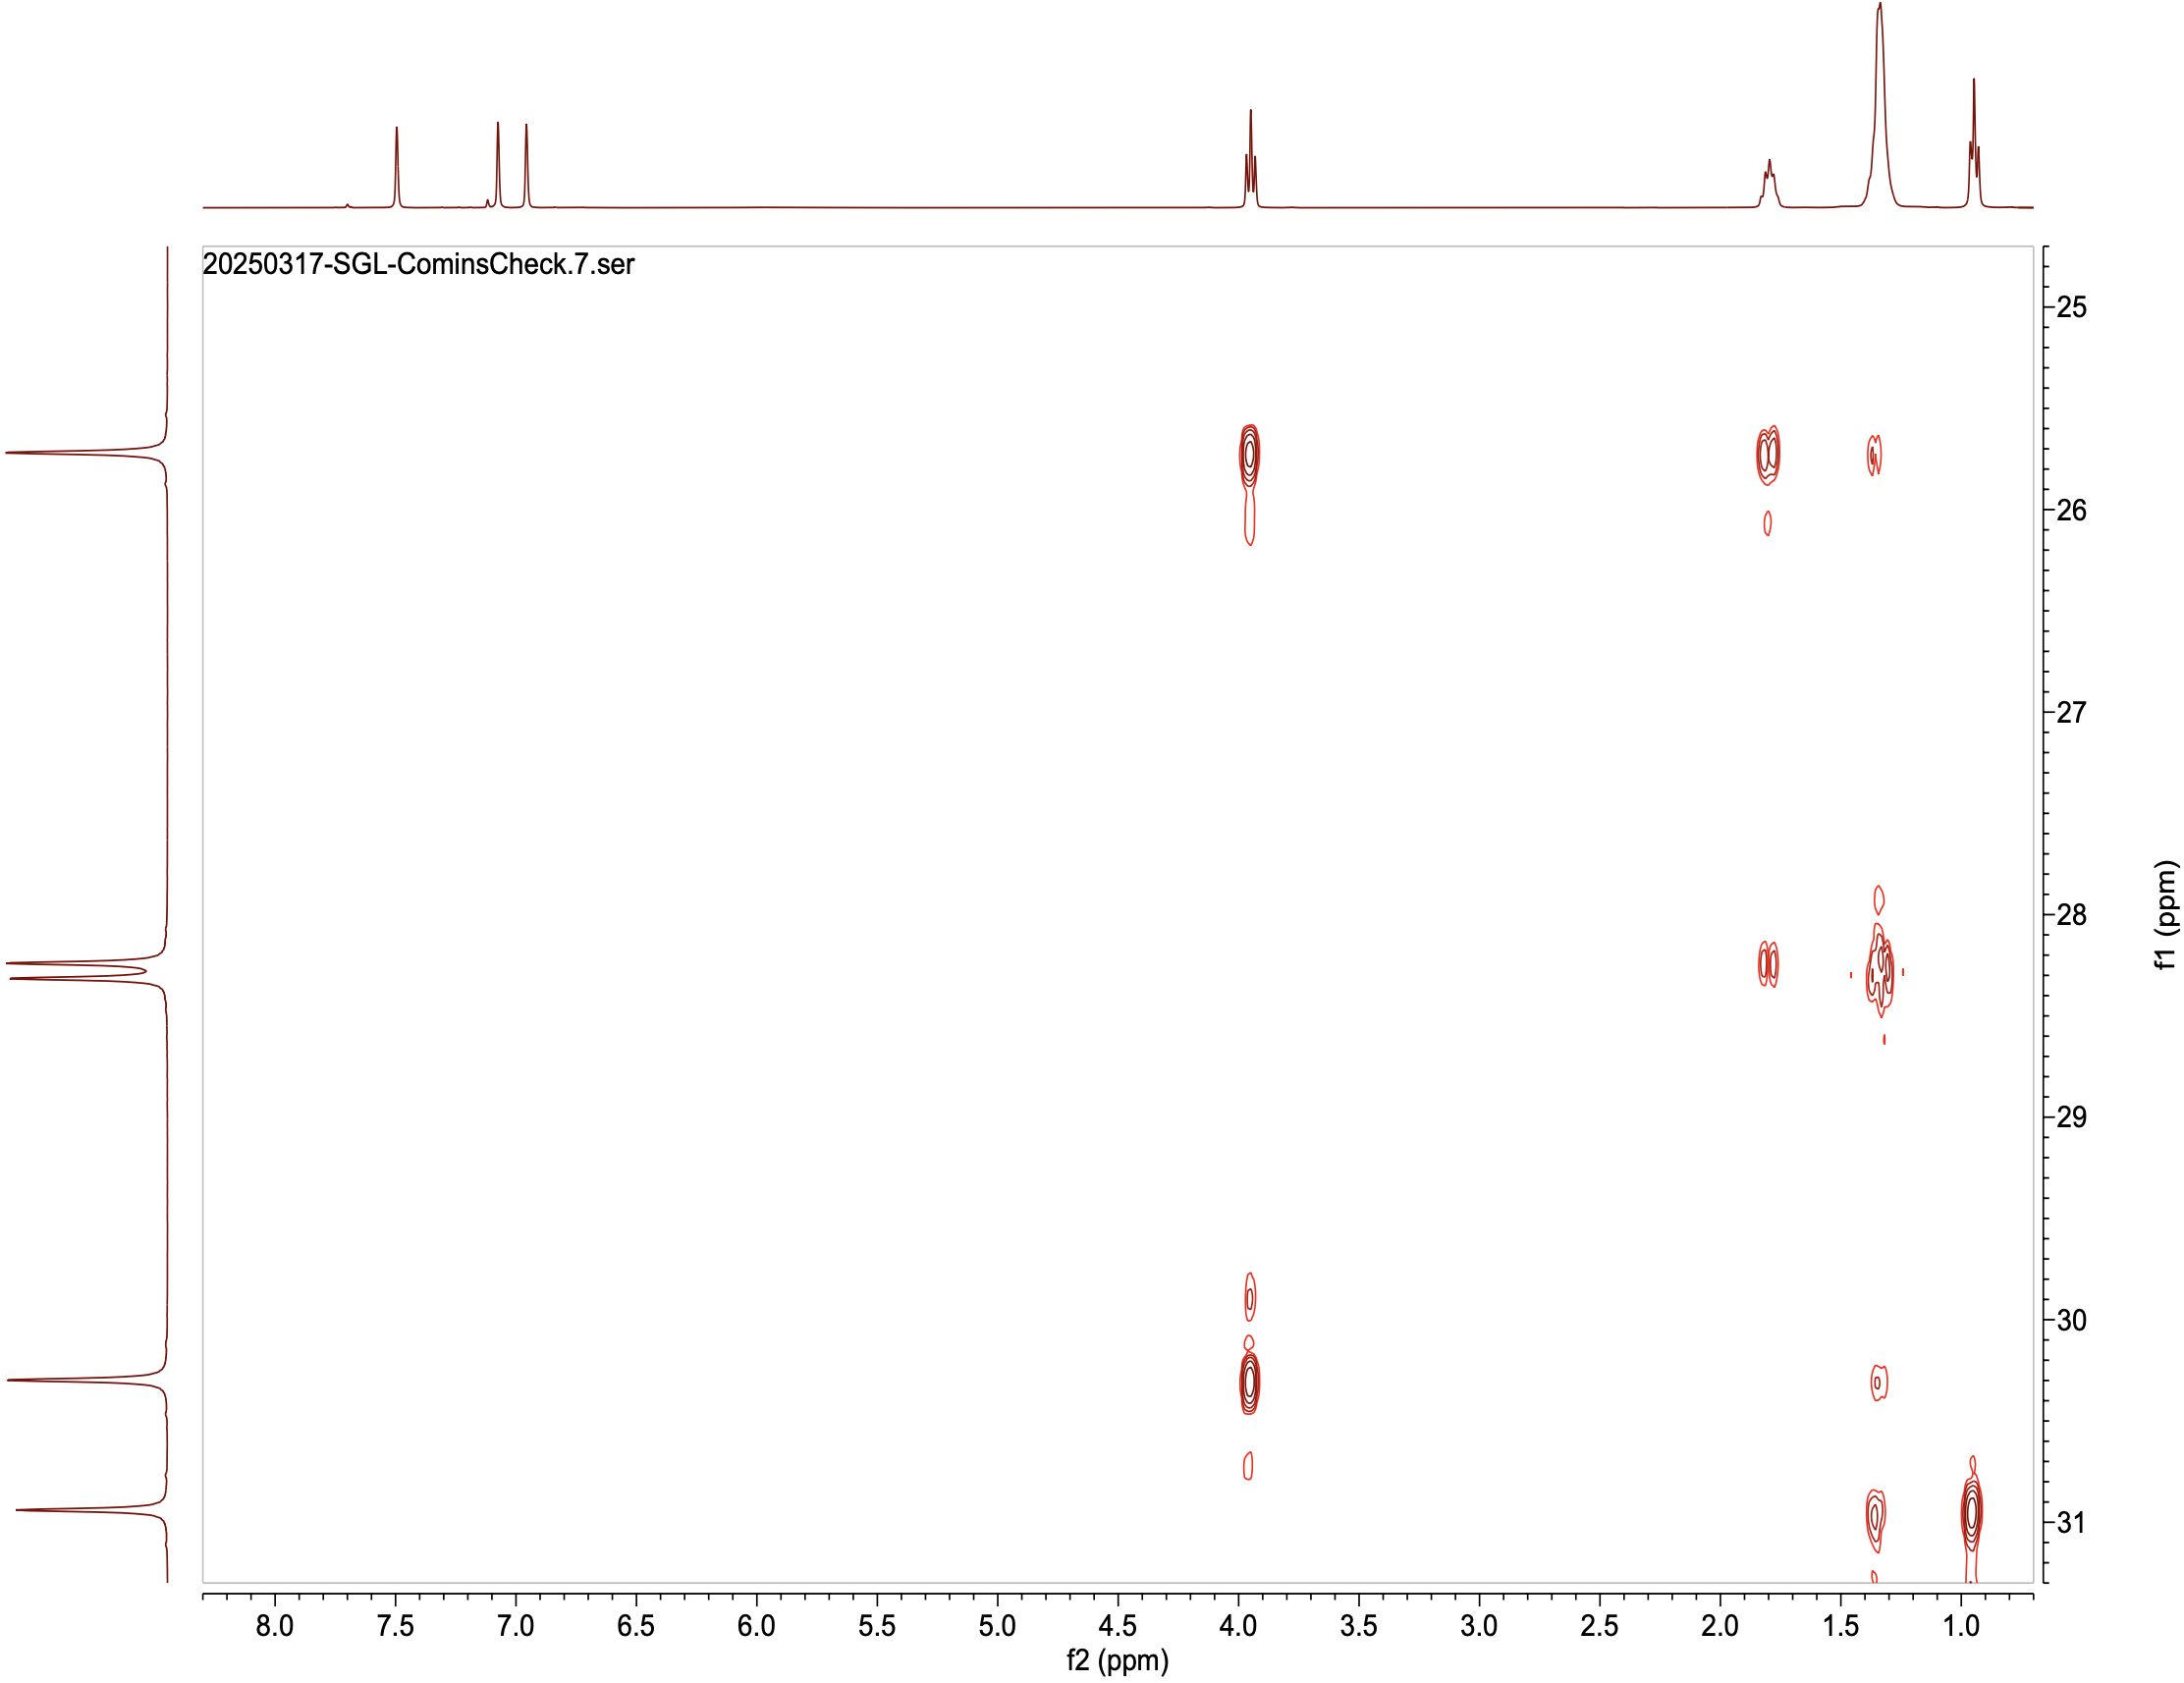
\includegraphics[width=\linewidth]{FPhmbcBand.png}
    \caption{Band-selective \ce{{}^1H}-\ce{{}^13C} HMBC spectrum of unknown, centered at \SI{28.28}{\partspermillion}.}
    \label{fig:FPhmbcBand}
\end{figure}
Fortunately, this spectrum did have the resolution to correlate the protons at \SI{1.80}{\partspermillion} with the carbon at \SI{28.24}{\partspermillion}. The last carbon (7) was thus assigned by process of elimination, and both of these carbons' protons were confirmed to be buried in the multiplet at \SI{1.34}{\partspermillion} by the HSQC correlations (see Figure \ref{fig:FPhsqc}).



\section{Additional Confirmational Experiments}
At this point, I feel content to accept the assignment of the unknown as 1-octylimidazole and of the proton and carbon peak assignments as those given in Figures \ref{fig:FP1H} and \ref{fig:FP13C}, respectively. However, I am cognizant that some assignments were based on chemical shift arguments when they need not be.\par
For example, a "smoking gun" to differentiate sites 1 and 3 in the imidazole ring would be a NOESY spectrum. Specifically, the (vicinal) protons 2 and 3 should have a NOESY cross peak. Note that 1-octylimidazole qualifies as low molecular weight, so ROESY is not necessary.\par
Going beyond the scope of 5.46, a "smoking gun" to differentiate 10 and 5 would be an HSQC-NOESY spectrum. Using this tool, we could correlate the 10 carbon (\SI{21.82}{\partspermillion}), through its proton, over to the vicinal protons in the terminal methyl group; the 5 carbon would not have such a correlation.



\section{Conclusion}
With the unknown compound's identity confirmed as 1-octylimidazole --- a quite precious substance that retails from MilliporeSigma\supercite{bib:FPSigma} at \$995 for one-fifth the quantity that I received --- I relabeled the container and entered the compound in my group's inventory.
\newpage



\printbibliography[heading=bibintoc]




\end{document}